\documentclass{elsarticle_nonatbib}\usepackage[]{graphicx}\usepackage[]{color}
%% maxwidth is the original width if it is less than linewidth
%% otherwise use linewidth (to make sure the graphics do not exceed the margin)
\makeatletter
\def\maxwidth{ %
  \ifdim\Gin@nat@width>\linewidth
    \linewidth
  \else
    \Gin@nat@width
  \fi
}
\makeatother

\definecolor{fgcolor}{rgb}{0.345, 0.345, 0.345}
\newcommand{\hlnum}[1]{\textcolor[rgb]{0.686,0.059,0.569}{#1}}%
\newcommand{\hlstr}[1]{\textcolor[rgb]{0.192,0.494,0.8}{#1}}%
\newcommand{\hlcom}[1]{\textcolor[rgb]{0.678,0.584,0.686}{\textit{#1}}}%
\newcommand{\hlopt}[1]{\textcolor[rgb]{0,0,0}{#1}}%
\newcommand{\hlstd}[1]{\textcolor[rgb]{0.345,0.345,0.345}{#1}}%
\newcommand{\hlkwa}[1]{\textcolor[rgb]{0.161,0.373,0.58}{\textbf{#1}}}%
\newcommand{\hlkwb}[1]{\textcolor[rgb]{0.69,0.353,0.396}{#1}}%
\newcommand{\hlkwc}[1]{\textcolor[rgb]{0.333,0.667,0.333}{#1}}%
\newcommand{\hlkwd}[1]{\textcolor[rgb]{0.737,0.353,0.396}{\textbf{#1}}}%

\usepackage{framed}
\makeatletter
\newenvironment{kframe}{%
 \def\at@end@of@kframe{}%
 \ifinner\ifhmode%
  \def\at@end@of@kframe{\end{minipage}}%
  \begin{minipage}{\columnwidth}%
 \fi\fi%
 \def\FrameCommand##1{\hskip\@totalleftmargin \hskip-\fboxsep
 \colorbox{shadecolor}{##1}\hskip-\fboxsep
     % There is no \\@totalrightmargin, so:
     \hskip-\linewidth \hskip-\@totalleftmargin \hskip\columnwidth}%
 \MakeFramed {\advance\hsize-\width
   \@totalleftmargin\z@ \linewidth\hsize
   \@setminipage}}%
 {\par\unskip\endMakeFramed%
 \at@end@of@kframe}
\makeatother

\definecolor{shadecolor}{rgb}{.97, .97, .97}
\definecolor{messagecolor}{rgb}{0, 0, 0}
\definecolor{warningcolor}{rgb}{1, 0, 1}
\definecolor{errorcolor}{rgb}{1, 0, 0}
\newenvironment{knitrout}{}{} % an empty environment to be redefined in TeX

\usepackage{alltt}
\usepackage[utf8]{inputenc}
\usepackage[T1]{fontenc}
\usepackage{lmodern} % load a font with all the characters
\usepackage[top=1in, left=1in, right=1in, bottom=1in]{geometry}

\usepackage{float, amsmath}
\usepackage{tikz}
\usetikzlibrary{shapes,arrows}
\usetikzlibrary{positioning}
\usepackage{float, amsmath}

\usepackage[hyphens]{url}
\usepackage{enumerate}
%\usepackage{chapterbib}
% \usepackage{natbib}
\usepackage{setspace} % delete when  \singlespacing is taken out 


\usepackage[
  natbib = true,
    backend=bibtex,
    isbn=false,
    url=false,
    doi=false,
    eprint=false,
    style=numeric,
    sorting=nyt,
    sortcites = true
]{biblatex}
\bibliography{ich_chapter}
\AtEveryBibitem{
\clearfield{note}
% \clearlist{address}
% \clearfield{eprint}
% \clearfield{isbn}
% \clearfield{issn}
% \clearlist{location}
% \clearfield{month}
% \clearfield{series}
} % clears language

\usepackage{hyperref}

\makeatletter
\providecommand{\doi}[1]{%
  \begingroup
    \let\bibinfo\@secondoftwo
    \urlstyle{rm}%
    \href{http://dx.doi.org/#1}{%
      doi:\discretionary{}{}{}%
      \nolinkurl{#1}%
    }%
  \endgroup
}
\makeatother

\newcommand{\pkg}[1]{\texttt{#1}}
\newcommand{\code}[1]{\texttt{#1}}

\usepackage{subfig}

\journal{NeuroImage}


%\usepackage[all]{hypcap}
\IfFileExists{upquote.sty}{\usepackage{upquote}}{}
\begin{document}



\graphicspath{{figures/}} % OK


\begin{frontmatter}

\date{}

\title{PItcHPERFeCT: Primary Intracranial Hemorrhage Probability Estimation using Random Forests on CT}
%\title{Validated Automatic Brain Extraction of Head CT Images using Established, Open-Source, Neuroimaging Software}



\auth[jhsph]{John~Muschelli\corref{cor1}}
\ead{jmusche1@jhu.edu}

\auth[jhsph]{Elizabeth~M.~Sweeney}
\ead{emsweene1@jhu.edu}

\auth[ucla]{Paul~Vespa}
\ead{PVespa@mednet.ucla.edu}

\auth[jhmi]{Daniel~F.~Hanley}
\ead{dhanley@jhmi.edu}

\auth[jhsph]{Ciprian~M.~Crainiceanu}
\ead{ccrainic@jhsph.edu}


\cortext[cor1]{Principal Corresponding Author}
\address[jhsph]{Department of Biostatistics, Bloomberg School of Public Health, Johns Hopkins University, Baltimore, MD, USA}
\address[jhmi]{Department of Neurology, Division of Brain Injury Outcomes,  Johns Hopkins Medical Institutions, Baltimore, MD, USA}
\address[ucla]{Department of Neurosurgery, David Geffen School of Medicine at UCLA, Los Angeles, CA, USA}












\begin{abstract}


\section*{Introduction}

Intracerebral hemorrhage (ICH), where a blood vessel ruptures into areas of the brain, accounts for approximately 10-15\% of all strokes.  X-ray computed tomography (CT) scans is largely used to assess the location and volume of the hemorrhage.

Manual segmentation of the CT scan using planimetry by an expert reader is the gold standard for volume estimation but is time-consuming and has within- and across-reader variability.  We propose an automated segmentation approach using a random forest algorithm with features extracted from X-ray computed tomography (CT) scans.  
\vspace{-1em}
\section*{Methods}
The Minimally Invasive Surgery and rt-PA in ICH Evacuation (MISTIE) trial was a multi-site Phase II clinical trial. We used $112$ patients from MISTIE, one CT scan per patient, using the first scan acquired.  ICH was manually segmented on CT scans by expert readers. We derived a set of imaging predictors from each scan. 

Using $10$ scans, we used a first-pass voxel selection procedure based on quantiles of a set of predictors and then built $4$ models estimating the voxel-level probability of ICH.  The models used were: 1) logistic regression, 2) logistic regression with a penalty on the model parameters using LASSO, 3) a generalized additive model (GAM) and 4) a random forest classifier.   We used $10$ scans for model estimation and $102$ scans for model validation.  

For each validation scan, the model predicted the probability of ICH, which was thresholded using a cutoff derived from the training data to a binary image mask.  This mask was compared to the manual segmentation mask using the correlation of the volume of the hemorrhage and the Dice Similarity Index (DSI), an overlap measure.  We tested equality of median DSI using the Kruskal-Wallis test and median pairs using the Wilcoxon rank-sum test. 

\vspace{-1em}

\section*{Results} 
The median DSI for each model was: $0.89$ (logistic), $0.885$  (LASSO), $0.88$ (GAM), and $0.899$ (random forest).  Using the random forest results in a slightly higher median DSI compared to the other models. After Bonferroni correction, the hypothesis of equality of median DSI was rejected only when comparing the random forest DSI to the DSI from the logistic ($p < 0.001$), LASSO ($p < 0.001$), or GAM ($p < 0.001$) models.  In practical terms the difference between the random forest and the logistic regression is quite small.  The correlation (95\% CI) between the volume from manual segmentation and the predicted volume was $0.932$ ($0.901, 0.954$) for the random forest model. These results indicate that the approach can achieve accurate segmentation of ICH in a population of patients from a variety of imaging centers.  

\end{abstract}

\begin{keyword}
CT \sep ICH Segmentation \sep Intracerebral Hemorrhage 
\end{keyword}

\end{frontmatter}


\renewcommand{\thesubfigure}{\Alph{subfigure}} % OK


\newcommand{\mywidth}{0.23}

\newcommand{\stubber}[1]{figures/Reseg_161-413_20110710_1619_CT_2_HEAD_Head#1.png}
%trim = 3in 10in 4in 3in, clip, 
\newcommand{\makeimg}[2]{\includegraphics[width=#1\linewidth]{\stubber{#2}}}





\section{Introduction}


%Bleeding may cause distension of the brain structures an increase in potentially lethal intracranial pressure (ICP).  ICH is a serious condition; it accounts for approximately 10-15\% of all strokes, corresponding to an estimated 79,500 annual cases \citep{go_heart_2013} and approximately 30,000 deaths \citep{qureshi_spontaneous_2001} in the US and approximately 5 million cases worldwide \citep{krishnamurthi_global_2014}. In addition to the increased likelihood of death, ICH has debilitating health effects on survivors who do not have full functional recovery after stroke.

Intracerebral hemorrhage (ICH) is a neurological condition that results from a blood vessel rupturing into the tissue and possibly the ventricles of the brain.   The use of X-ray computed tomography (CT) scans allows clinicians and researchers to qualitatively and quantitatively describe the characteristics of a hemorrhage to guide interventions and treatments.  CT scanning is widely available and is the most commonly used diagnostic tool in patients with ICH \citep{sahni_management_2007}.  The volume of ICH has been consistently demonstrated to be an important diagnostic predictor of stroke severity, long-term functional outcome, and mortality \citep{broderick_volume_1993, hemphill_ich_2001, tuhrim_volume_1999}.  ICH volume change is also common primary outcome \citep{anderson_intensive_2008, anderson_effects_2010, qureshi_association_2011, mayer_recombinant_2005} and secondary outcome \citep{morgan_preliminary_2008_mistie, anderson_intensive_2008, morgan_preliminary_2008_clear} in clinical trials.  Moreover, the location of the ICH has been shown to affect functional outcome in patients with stroke \citep{rost_prediction_2008, castellanos_predictors_2005}.

ICH volume can be estimated quickly, for example,  using the ABC/2 method \citep{broderick_volume_1993}.  In this method, a reader chooses the slice with the largest area of hemorrhage.  The length of the intersection between this first axis and the hemorrhage is denoted by A. The next step is to draw an orthogonal line  at the middle of the segment of length A in the same plane that contains the largest hemorrhage area. The length of the intersection between this second orthogonal axis and the hemorrhage is denoted by B.  The reader then counts the number of slices where hemorrhage is present (C).  The volume estimate is $\frac{A\times B\times C}{2}$, which is an approximation of the volume under the assumption that the hemorrhage shape is well approximated by an ellipsoid \citep{kothari_abcs_1996}.  As this method is relatively easy to implement in practice, it can be used to quickly produce estimates of hemorrhage volume. 

Although ABC/2 is widely used, \citet{divani_abcs_2011} found that the measurement error associated with the ABC/2 method were significantly greater than those using planimetry, which requires slice-by-slice hemorrhage segmentation by trained readers. Planimetry is much more labor intensive and time consuming, but it tends to significantly outperform the ABC/2 approach, especially for irregularly shaped ICH and for smaller thickness (i.e.~higher resolution) scans.  Recently, \citet{webb_accuracy_2015} found that ABC/2 measurements at a clinical site, 81\% of the $4,369$ scans were within 5 milliliters (mL) of ICH volume compared to planimetry methods, but only 41\% were within 20\%.   Another problem that has not been discussed in the literature is that ICH may change over time. The shape of the ICH may initially be well approximated by an ellipsoid but the approximation may become increasingly inaccurate over time as the lesion changes shape, migrates through the surrounding tissues, or breaks down.  Surgical interventions that target the removal of ICH may also change the shape of the ICH or cause additional bleeding. This is particularly worrying in clinical trials where the ICH exposure may be measured with substantial bias and reduce the power of the tests.  An additional problem is that the ABC/2 method does not take into account intraventricular hemorrhage (IVH), which has been shown to be prognostic of 30-day mortality \citep{hemphill_ich_2001, tuhrim_volume_1999}.  Moreover, the ABC/2 method has been shown to consistently over-estimate infarct volume \citep{pedraza_reliability_2012} and may have significant inter-rater variability \citep{hussein_reliability_2013}. Therefore, a rapid, automated, and validated method for estimating hemorrhage location and its volume from CT scans is highly relevant in clinical trials and has both diagnostic and prognostic value.

Methods have been proposed for segmentation of ICH using magnetic resonance images (MRI) \citep{wang_hematoma_2013, carhuapoma2003brain}.  However, in most clinical settings,
the protocol is not standardized for MRI scans.  MRI sequences and protocols may vary across sites and there is no general, standardized, agreed-upon MRI modality for ICH standard-of-care.
Thus, there is a need for ICH segmentation that relies only on CT scan information, is reliable, reproducible, available, and well validated against planimetry.

We propose an algorithm that can estimate the probability of ICH at the voxel level, a binary ICH image, and the ICH volume.  We will compare our predicted ICH maps to the gold standard -- manual segmentation.  Several methods have been presented for automated methods for estimating ICH from CT scans \citep{ gillebert_automated_2014, prakash_segmentation_2012, loncaric_hierarchical_1996, loncaric_quantitative_1999, perez_set_2007}.  These methods include fuzzy clustering \citep{prakash_segmentation_2012, loncaric_hierarchical_1996}, simulated annealing \citep{loncaric_quantitative_1999}, 3-dimensional (3D) mathematical morphology operations \citep{perez_set_2007}, and template-based comparisons \citep{gillebert_automated_2014}.  Unfortunately, no software for ICH segmentation is publicly available.   The only software that we were able to obtain after requesting it was the one presented in \citet{gillebert_automated_2014}. This software requires a moderate level of technical knowledge.  We provide a completely automated pipeline of analysis from raw images to binary hemorrhage masks and volume estimates, and provide a public webpage to test the software. 

\section{Methods}

\subsection{Data} 
\subsection{ Participants and Imaging Data }
We used CT images from patients enrolled in the MISTIE (Minimally Invasive Surgery plus recombinant-tissue plasminogen activator for Intracerebral Evacuation) stroke trial \citep{morgan_preliminary_2008_mistie}. We analyzed $112$ scans taken prior to randomization and treatment, corresponding to the first scan acquired post-stroke for $112$ unique patients.  Inclusion criteria into the study included: $18$ to $80$ years of age, spontaneous supratentorial intracerebral hemorrhage above $20$ milliliters (mL) in size (for full criteria, see \citet{mould_minimally_2013}).  The population analyzed here had a mean (SD) age was $60.7$ $(11.2)$ years, was $68.8\%$ male, and was 53.6\% Caucasian, 31.2\% African American, 10.7\% Hispanic, and 4.5\% Asian or Pacific islander.  CT data were collected as part of the Johns Hopkins Medicine IRB-approved MISTIE research studies with written consent from participants.  

% Do not wrap $ in man.tab. 
The study protocol was executed with minor, but important, differences across the $26$ sites.  Scans were acquired using $4$ scanner manufacturers: GE ($N=46$),  Siemens ($N=38$),  Philips ($N=20$),  and Toshiba ($N=8$).   In head CT scanning, the gantry may be tilted so that sensitive organs, such as the eyes, are not exposed to X-ray radiation.  This causes scan slices to be acquired at an oblique angle with respect to the patient.  Gantry tilt was observed in $88$ scans.
%n.gant scans.  
Slice thickness of the image varied within the scan for 14 scans.
%n.var.slice scans. 
For example, a scan may have $10$ millimeter (mm) slices at the top and bottom of the brain and $5$mm slices in the middle of the brain.  Therefore, the original scans analyzed had different voxel (volume element) dimensions.  These conditions are characteristic of how scan are presented in many diagnostic cases.

% All CT scans used in template creation were acquired on the same Siemens Sensation 64, peak 120 kV, 348 mA X-ray Tube Current. The reconstructed resolution of all the images ranged from 0.69 × 0.69 × 0.5 mm to 0.45 × 0.45 × 0.5 mm with full brain coverage. 


\subsection{Hemorrhage Segmentation and Location Identification}
ICH was manually segmented on CT scans using the OsiriX imaging software by expert readers (OsiriX v. 4.1, Pixmeo; Geneva, Switzerland).  Readers employed a semiautomated threshold-based approach using a Hounsfield unit (HU) range of $40$ to $80$ to select potential regions of ICH \citep{bergstrom_variation_1977, smith_imaging_2006}; these regions were then further quality controlled and refined by readers using direct inspection of images.  Binary hemorrhage masks were created by setting voxel intensity to $1$ if the voxel was classified as hemorrhage, regardless of location, and $0$ otherwise.  
%previous to this analysis as a standard hemorrhage characteristic.

\subsection{Image Processing: Brain Extraction, Registration}
CT images and binary hemorrhage masks were exported from OsiriX to DICOM (Digital Imaging and Communications in Medicine) format.   The image processing pipeline can be seen in Figure~\ref{fig:framework}.   Images with gantry tilt were corrected using a customized MATLAB (The Mathworks, Natick, Massachusetts, USA) user-written script ({\scriptsize \url{http://bit.ly/1ltIM8c}}). Images were converted to the Neuroimaging Informatics Technology Initiative (NIfTI) data format using \code{dcm2nii} (provided with MRIcro \citep{rorden_stereotaxic_2000}).  Images were constrained to values $-1024$ and $3071$ HU to remove potential image rescaling errors and artifacts.   No interpolation was done for images with a variable slice thickness. Thickness was determined from the first converted slice and the NIfTI format assumes homogeneous thickness throughout the image.  
% This loss of information, if not properly accounted for, affects volume estimation, which relies on accurate pixel dimensions in millimeters.  Variable slice thickness should have no affect on the other estimates of performance described below, such as sensitivity, as they are calculated at a voxel level and do not rely on pixel resolution.  Although the NIfTI images store the data with only one pixel dimension for the height of the voxel, we use the ImagePositionPatient DICOM field to determine the accurate height of each voxel to calculate an accurate volume.  

All image analysis was done in the R statistical software \citep{RCORE}, using the \pkg{fslr} \citep{muschelli2015fslr} package to call functions from the FSL \citep{jenkinson_fsl_2012} neuroimaging software (version 5.0.4), and the \pkg{ANTsR} package to call functions from the ANTs (Advanced Normalization Tools) neuroimaging software \citep{avants_reproducible_2011}.

Brains were extracted to remove skull, eyes, facial and nasal features, extracranial skin, and non-human elements of the image captured by the CT scanner, such as the gantry, pillows, or medical devices.  Removal of these elements was performed using the brain extraction tool (BET) \citep{smith_fast_2002}, a function of FSL, using a previously published validated CT-specific brain extraction protocol \citep{muschelli_validated_2015}.  

%Different reconstructions of CT images are not available via the data-acquiring center, and 


\tikzstyle{bblock} = [rectangle, draw, text width=8em, text centered, minimum height=2em, rounded corners]
\tikzstyle{line} = [draw, text centered , -latex']
\tikzstyle{line node} = [draw, fill=white, font=\tiny ]
\tikzstyle{block} = [rectangle, draw, text width=5em, text centered, minimum height=4em, rounded corners]    
%
%\begin{figure}
%\centering
%\begin{tikzpicture}[node distance = 1.5cm, every node/.style={rectangle,fill=white}, scale=0.75, transform shape]
% Place nodes
%\node [bblock] (raw) {DICOM images};
%\node [bblock, below = 2.5cm of raw] (dcmnii) {NIfTI image};
%\node [bblock, below of=dcmnii] (thresh) {Threshold to 0-100 HU };
%\node [bblock, above right=1cm and 1.25cm of dcmnii] (gantry) {Gantry tilt correction};
%\node [bblock, below of=thresh] (BET) {BET for CT};
%
%\node [block, below left=2cm and -4em of BET] (native) {Native Image};
%\node [block, left = 1.5em of native] (n4) {N4 Correction};
%\node [block, left = 1.5em of n4] (n3) {N3 Correction};
%\node [block, right = 1.5em of native] (rigid) {Rigid Registration};
%\node [block, right = 1.5em of rigid] (affine) {Affine Registration};
%\node [block, right = 1.5em of affine] (syn) {SyN Registration};
%
%\node [bblock, below right=1.5cm and -4em of native] (predictors) {ICH Predictors};
%
%
%\node [bblock, below of=predictors] (Models) {Prediction Models};
%
%\node [bblock, below of=Models] (Measures) {Performance Measures};
%
%\node [bblock, above right=.2cm and .6cm of Measures] (smooth) {Smoothed predictions};
%
%
% Draw edges
%\path [line] (raw) -- node {dcm2nii} (dcmnii);
%\path [line] (raw) -- (gantry);
%\path [line] (gantry) -- node {dcm2nii} (dcmnii);
%\path [line] (dcmnii) -- (thresh);
%\path [line] (thresh) -- (BET);
%\path [line] (BET) -- (syn);
%\path [line] (BET) -- (n3);
%\path [line] (BET) -- (n4);
%\path [line] (BET) -- (affine);
%\path [line] (BET) -- (rigid);
%\path [line] (BET) -- (native);
%\path [line] (BET) -- node {Different Processing Pipelines} (native);
%
%\path [line] (BET) -- node {Inhomogeneity Correction} (n3);
%
%\path [line] (BET) -- node {Registration} (affine);
%
%\path [line] (native) -- (predictors);
%\path [line] (affine) -- (predictors);
%\path [line] (rigid) -- (predictors);
%\path [line] (syn) -- (predictors);
%\path [line] (n3) -- (predictors);
%\path [line] (n4) -- (predictors);
%
%\path [line] (predictors) -- (Models);
%\path [line] (smooth) -- (Measures);
%\path [line] (Models) -- (smooth);
%\path [line] (Models) -- (Measures);
%\end{tikzpicture}
%\caption{{\bf Processing Pipeline}.  Images in DICOM (Digital Imaging and Communications in Medicine) format were gantry tilt corrected if necessary and converted to NIfTI (Neuroimaging Informatics Technology Initiative) format using \texttt{dcm2nii}.  After NIfTI conversion, the data is thresholded to tissue ranges of $0$-$100$ Hounsfield units (HU).  BET was applied to the image using a previously published protocol.  Different image registration techniques and inhomogeneity correction methods were derived from the native image.  Imaging predictors were created and used in logistic regression models. }
%\label{fig:framework}
%\end{figure}


\begin{figure}
\centering
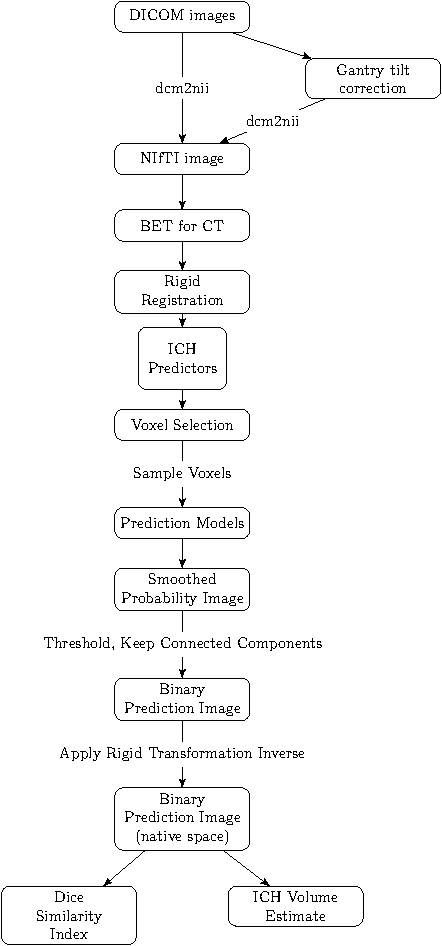
\includegraphics[width=0.5\linewidth]{Imaging_Pipeline_Flowchart_with_Rigid.pdf}
\caption{{\bf Processing Pipeline}.  Images in DICOM (Digital Imaging and Communications in Medicine) format were gantry tilt corrected if necessary and converted to NIfTI (Neuroimaging Informatics Technology Initiative) format using \texttt{dcm2nii}.  After NIfTI conversion, the brain extraction tool (BET) was applied to the image using a previously published protocol.  The image was rigidly registered to a brain CT template.  We estimated imaging predictors and used these predictors to estimate the probability of ICH in a prediction model.  The probability of ICH was thresholded, connected component below $100$ voxels ($0.1$mL) were discarded, and the image was transformed back into original space of the patient.  The ICH volume and the Dice Similarity Index, an overlap measure, were calculated compared to the true estimate from the manual segmentation.  }
\label{fig:framework}
\end{figure}

\subsection{Image Registration}
\citet{rorden_age-specific_2012} introduced a CT template based on $35$ individuals who presented with specific neurological deficits that were suspected to be caused by a stroke, but were later found to be due to a metabolic abnormality.  This CT template is represented in MNI (Montreal Neurological Institute) space and brain-extraction was performed on the template.  Prior to image processing, brain-extracted images were registered to this brain-extracted template using a rigid-body (6 degrees of freedom) and linearly interpolated to a $1\times1\times1$mm voxel resolution.  Transformed hemorrhage masks and brain masks were thresholded using a value of $0.5$ to preserve mask volume \cite{flirt_reg}. This operation reoriented the image, ensured isotropic voxel sizes for smoothing and other operations described below, and preserved the relative volume of the ICH.  All image preprocessing and analysis are done in MNI space, described as template space, unless otherwise specified.


\subsection{Brain Mask Erosion}
Each brain mask was eroded by a box kernel ($3\times3\times1$mm).  Though this erosion may exclude voxels from superficial bleeds towards the cortical surface, it excludes voxels with similar ranges as ICH voxels, caused by 1) incomplete skull stripping or 2) partial voluming effects with the skull.  If any voxels from the hemorrhage mask was removed due to brain extraction or brain mask erosion, these voxels were included in estimating model performance but their predicted probability of ICH was set to $0$.  Therefore, these deleted ICH voxels will always be incorrectly predicted by our approach as not ICH.  

%This eroded mask and any excluded ICH voxels contained all voxels used for exploratory analysis and model fitting, which we will refer to as candidate voxels.



\subsection{Imaging Predictors}
\label{sec:predictors}
We derived a set of imaging predictors from each CT scan.  We will describe each predictor together with the rationale for their use.  These features make up the potential set of predictors (features) for image segmentation.  Below we provide the definition of thess predictors, while Figure~\ref{fig:pred} displays them for one axial slice of one subject. 
%Note that the corresponding images have roughly a distribution of between $0$ and $100$ HU as they have been skull stripped.  

\subsubsection{CT voxel intensity information} The first predictor is the raw voxel intensity value in HU denoted by $x(v)$. This is the main predictor used in visual inspection, with high HU values being indicative of hemorrhage. Based on the voxel intensity we have also created an indicator for the HU intensity value to be between $40$ and $80$ (inclusive), to mimic the criterion used for screening in manual segmentation. More precisely, we have introduced the predictor $$
I_{\text{thresh}}(v) = \begin{cases}
1 & \text{if } 40 \leq x(v) \leq 80 \\
0 & \text{otherwise}
\end{cases}
$$. 

\subsubsection{Local Moment Information} For each voxel, we extracted a neighborhood, denoted $N(v)$, of all adjacent voxels along the $3$ dimensions together with the voxel itself.  If $x_k(v)$ denotes the voxel intensity in HU for voxel neighbor $k$, where $k = 1, \dots, N(v) = 27$, then the local mean intensity is defined as:
\begin{equation}
\bar{x}(v) = \frac{1}{N(v)} \sum_{k \in N(v)} x_k(v). \label{eq:mean}
\end{equation}
Based on similar ideas we have also calculated statistics based on higher order moments and define the local standard deviation (SD), skew, and kurtosis as:
\begin{eqnarray*}
\text{SD}(v) &=& \sqrt{ \frac{1}{N(v)} \sum_{k \in N(v)} \left\{x_k(v) - \bar{x}(v)\right\}^2 } \\
\text{Skew}(v) &=& \frac{ \frac{1}{N(v)} \sum\limits_{k \in N(v)} \left\{x_k(v)-\bar{x}(v) \right\}^3 } {\left[ \frac{1}{N(v)} \sum\limits_{k \in N(v)} \left\{x_k(v)- \bar{x}(v)\right\}^2\right]^{3/2}} \\
\text{Kurtosis}(v) &=& \frac{ \frac{1}{N(v)} \sum\limits_{k \in N(v)} \left\{x_k(v)- \bar{x}(v)\right\}^4 }{ \left[ \frac{1}{N(v)} \sum\limits_{k \in N(v)} \left\{x_k(v)- \bar{x}(v)\right\}^2\right]^2} \\
\label{eq:moment}
\end{eqnarray*}
We did not divide by $\{N(v) - 1\}$ in standard deviation and skew formula and did not subtract by $3$ for kurtosis.  As $N(v)$ is the same at every voxel, these simplified choices will have no effect on modeling or prediction. 


Voxels with a larger local mean have higher HU neighboring voxels, which increases their likelihood to be in or adjacent to the ICH.  The higher order moments can provide information about how homogeneous the intensities in the neighborhood are and where edges may be located.  We also introduce the variable of the percentage of voxels in each neighborhood that have HU values between $40$ and $80$:
\begin{equation}
p_{\text{thresh}}(v) = \frac{1}{N(v)} \sum_{k \in N(v)} I\{ 40 \leq x_k(v) \leq 80 \} \label{eq:pct}
\end{equation}
which should be higher for ICH voxels as they are surrounded by neighbors with higher HU values.  

Voxels that are on the surface or are surrounded by non-brain tissue are less likely to be in the ICH.  Thus, voxels not in eroded mask are set to $0$.    
We also introduce the variable percentage of voxels that have neighbors of value of $0$:
\begin{equation}
p_{0}(v) = \frac{1}{N(v)} \sum_{k \in N(v)} I\{ x_k(v) = 0 \}, \label{eq:pct0}
\end{equation}
and an indicator of whether any voxels in the neighborhood had a value of $0$:
\begin{equation}
\bar{I}_{0}(v) = I\{ p_{0}(v) > 0 \}. \label{eq:I0}
\end{equation}

The reason for introducing these predictors is that we expect that voxels that have neighbors with intensity zero are less likely to be ICH. Our approach will not assume that the probability of voxels with neighbors with HU intensity equal to zero are not in the ICH. Instead, we will model the probability of belonging to the ICH as a function of the predictors described in this section. 
 
\subsubsection{Within-plane Standard Scores} Some brain structures have high HU values but are not ICH, such as the falx cerebri, which lies largely on the mid-sagittal plane.  Moreover, raw CT images may contain substantial inhomogeneity. For example, tissues closer to the top of the brain may have a higher observed intensities (measured in HU) than those in the middle or bottom of the brain.  Thus, if values are standardized within each plane (axial, sagittal, coronal), the resulting plane-specific z-scores may discriminate better high relative values within the plane, which may attenuate the effect of low-frequency HU intensity inhomogeneities.

Thus, for each voxel and slice (axial, sagittal, and coronal) planes, we defined 
\begin{equation}
z_{o}(v) = \frac{x(v) - \bar{x}(v, o)}{\sigma(v, o)} \label{eq:z}
\end{equation}
where $o \in \{$axial, sagittal, and coronal$\}$, $\bar{x}(v, o)$ and $\sigma(v, o)$ denote the mean and standard deviation of the intensities of voxels in the plane $o$ that contains the voxel $v$, excluding voxels outside the brain mask.   In addition to the standardized images within each plane we have also calculated standardized scores based on the Winsorized mean and standard deviation.  More precisely, we calculated the same formula as in equation~\eqref{eq:z}, but used only voxels with HU values between the 10th and 90th percentile of intensity within the slice to calculate the slice-specific mean and standard deviation. This approach is expected to be more robust to small and moderate artifacts in the image.. 

\subsubsection{First-pass Segmentation} A major advantage of our approach is that it can use the results of other segmentation algorithms as covariates in our model. Consider, for example, Atropos \citep{atropos}, a previously published, open source, general segmentation tool based on Markov random fields for image segmentation.  We used used Atropos to conduct a 4-tissue class segmentation and combined the top 2 probability classes into one class.  The probability of the resulting class was then used a predictor, denoted by $\text{Atropos}(v)$.  Although Atropos has been shown to perform well in other studies for tissue-class segmentation \citep{atropos, menze2015multimodal}, the Atropos segmentation did not perform adequately in our ICH CT data. However, using the Atropos segmentation probabilities as predictors can be done seamlessly in our approach. Similarly, the results of any other segmentation approach can be incorporated in our approach and the relative performance of methods can be compared.

\subsubsection{Contralateral Difference Images}  As most hemorrhages are constrained to one side of the brain, the contralateral side tends to have lower HU values.  In contrast, for non-hemorrhage voxels, the contralateral voxels tend to have similar HU values due to the quasi-symmetry of the brain. To take advantage of this property, we right-left flipped the image, and computed a difference image 
\begin{equation}
f(v) = x(v) - x(v^{*}), \label{eq:flip}
\end{equation}
where $v^{*}$ is the contralateral voxel of $v$.  



\subsubsection{Global Head Information} Another potential predictor was the distance to the center of the brain, $d(v)$, account for voxels that are far from the brain center but may contain artifacts.  We also created $3$ images by smoothing the original image using large Gaussian kernels ($\sigma = 5mm^3, 10mm^3, 20mm^3$) to account for potential heterogeneity in intensity. These smooth images we denoted by $s_{5}(v)$, $s_{10}(v)$ and $s_{20}(v)$, respectively.   

\subsubsection{Standardized-to-template Intensity}  
We have also incorporated predictors that contrast the scan HU intensities with those of an average brain obtained from healthy individuals.  Using $30$ CT images from non-stroke patients from Dr.~Rorden (personal communication), we registered the brain-extracted scans to a CT template, and created a voxel-wise mean image $M$ and voxel-wise standard deviation $S$ image across registered images in template space.  Each scan in our ICH study, we registered (using affine transformations followed by SyN \citep{avants_symmetric_2008}) it to the same CT template. We then  created a standardized voxel intensity with respect to this population, $z_{\text{template}}$, using the following equation:
$$
z_{\text{template}}(v) = \frac{x(v) - M(v)}{S(v)}
$$
The image was then warped back into the original space to align this predictor with the other predictors.  This predictor is similar to that used in \citet{gillebert_automated_2014}.  


%Although standardizing voxels compared to within-scan measurements can detect anomalous tissue, one powerful tool is to use a measure how different a voxel is compared to that voxel in a person from a non-stroke population.  We registered the brain-extracted image to the brain-extracted CT template using an affine transformation, followed by a non-linear transformation estimated using Symmetric Normalization (SyN) \citep{avants_symmetric_2008}.  


\begin{figure}
\centering
\begin{center}
\begin{tabular}{@{}c@{}c@{}c@{}c@{}}
$x(v)$ & Atropos$(v)$ & $f(v)$ & $d(v)$ \\
\makeimg{\mywidth}{_SS} & \makeimg{\mywidth}{_prob_img} & \makeimg{\mywidth}{_flipped_value}   & \makeimg{\mywidth}{_dist_centroid} \\
$\bar{x}(v)$ & $\text{SD}(v)$ & $\text{Skew}(v)$ & $\text{Kurtosis}(v)$\\
\makeimg{\mywidth}{_moment1} & \makeimg{\mywidth}{_moment2} &  \makeimg{\mywidth}{_skew} &  \makeimg{\mywidth}{_kurtosis}\\
$p_{0}(v)$ & $\bar{I}_{0}(v)$  & $p_{\text{thresh}}(v)$ & $I_{\text{thresh}}(v)$\\
\makeimg{\mywidth}{_pct_zero_neighbor} & \makeimg{\mywidth}{_any_zero_neighbor} & \makeimg{\mywidth}{_pct_thresh_40_80} & \makeimg{\mywidth}{_thresh_40_80}   \\
$s_{5}(v)$ & $s_{10}(v)$  & $s_{20}(v)$& $z_{\text{template}}(v)$ \\
\makeimg{\mywidth}{_smooth5}  & \makeimg{\mywidth}{_smooth10} & \makeimg{\mywidth}{_smooth20} & \makeimg{\mywidth}{_zscore_template} 
\end{tabular}
\end{center}
\caption{{\bf Predictor Images}. Here we display one slice from one patient for predictor images.  
The within-plane standardized and Winsorized predictor images were not shown as they are within-subject scaled versions of the image $x(v)$ and appear very similar.  Although they appear similar at a subject level, the distribution of these predictors is different across patients.  Images that visually separate the areas of ICH compared to the rest of the images are likely to be better predictors. 
}
\label{fig:pred}
\end{figure}




%To further illustrate how smoothing affects brain extraction, we present one example case where brain extraction performance with BET was acceptable only after smoothing.  





\subsection{Voxel Selection Procedure}
\label{sec:voxsel}
We chose $10$ scans from $10$ patients to perform exploratory data analysis, model fitting, and estimation of model cutoffs; these data will be referred to as the training data. We used the $102$ remaining scans as test data to evaluate the performance of the proposed approaches.
%Of the non_nmods remaining scans, we split the data into $groups["Validation"]$ validation scans and  $groups["Test"]$ test scans.  


Using the training data we estimated the $0.5\%$ and $99.5\%$ quantiles for all predictors across ICH voxels. The voxel selection procedure consisted of choosing all voxels that had all of predictors $z_{\text{axial}}$, $z_{\text{coronal}}$, and $p_{\text{thresh}}$ within the corresponding $0.5$ and $99.5$ quantiles as well as values of HU intensity between $30$ and $100$. Voxels that did not meet these criteria were assigned a $0$ probability of ICH. These cutoffs were found empirically to work well in the test scans. This approach excluded a mean of  63.6 (min: 37.1, max: 89.8) percentage of non-ICH voxels and included a mean of 97.9 (min: 91.6, max: 99.9) percentage of ICH voxels.  We have found that this voxel selection procedure improves computational speed as well as the performance of the algorithms.  

\subsection{Models}
\label{sec:mods}
Using the $10$ training scans we obtained all voxels passing the voxel selection procedure described in Section~$\ref{sec:voxsel}$.  We then randomly sub-sampled $100{,}000$ voxels, which were used for model fitting and selection as well as to conduct data exploratory analysis.  The rest of the remaining voxels were used for model calibration and testing.   All models were fit with all the predictors described in Sections~\ref{sec:predictors}.  

% get Reseg_Aggregate_data Rda for nunmber of voxels 

We fit several different models on the $100{,}000$ sub-sampled voxels: 1) logistic regression with all covariates used as main effects (without interactions or nonlinear effects), 2) logistic regression model with a penalty on the model parameters to reduce the potential effect of high correlations between predictors, 3) generalized additive model (GAM) \citep{hastie_generalized_1986, hastie_generalized_1990}, which is similar to the logistic regression, but allows for non-linear effects on the linear predictor scale, and 4) random forest classifier \citep{breiman2001random}.  All models were fit using R.

For the standard and penalized logistic regression model, we used all predictors.  The penalized model was fit using the LASSO (Least Absolute Shrinkage and Selection Operator) penalty \citep{tibshirani_regression_1996} using the \pkg{glmnet} package \citep{friedman_regularization_2010}.  The tuning parameter, $\lambda$, was chosen using 10-fold cross-validation on the training voxels; the cost function used was the misclassification rate.  The parameter was chosen using the largest value of $\lambda$ where that the misclassification rate is within 1 standard error of its minimum; this approach led to superior out-of-sample stability.

The generalized additive model (GAM) \citep{hastie_generalized_1986, hastie_generalized_1990} was also created using indicator variables for binary variables and thin-plate splines for all continuous measures. The model was fit using fast-estimation of the restricted maximum likelihood (fREML) implemented in the \pkg{mgcv} package \citep{wood_fast_2011, wood_generalized_2015}.   Detailed model specifications are provided in Section~\ref{sec:modspec}.


The random forest \citep{breiman2001random} classification algorithm was implemented using the \pkg{randomForest} package in R \citep{randomForest} with the default pruning parameters and number of trees (\code{ntree=500}, \code{mtry=4}). 



\subsection{Estimating a Cutoff for Model Probability}
\label{sec:cutoffs}
Each model described in Section~\ref{sec:mods} provides an estimate of the probability for each voxel to be in ICH.  For each model, the probability image was smoothed by taking the average over the neighborhood voxels (1 voxel in every direction).  These smooth maps were used to produce binary ICH maps by thresholding the probability of being in the ICH. Thus, the performance of methods depends strongly on the choice of these thresholds.

To choose the probability thresholds, we used the voxels in the training data that were not used for estimating the model.  Based on these voxels in the smoothed images, we estimated the probability cutoffs that minimized the Dice Similarity Index (DSI) \citep{dice_measures_1945} between the predicted ICH region at a particular threshold and the hand-segmented ICH.  
 The DSI is measure of overlap that is insensitive to areas where neither the true nor the predicted segmentation were labeled ICH, and will be used as a performance measure when comparing models on the test data.  DSI for scan $i$ is calculated by 
 $$
 DSI_i = \frac{2 \times TP}{2\times TP + FN + FP}
 $$
Here $TP$ denotes the number of ``true positive'' voxels, where the manual and predicted segmentation 
agree that the voxel is in ICH, $FP$ denotes the number of ``false positive'' voxels, where the predicted segmentation indicates that there is no lesion when the manual segmentation indicates lesion, and $FN$ denotes the number of ``false negative'' voxels, where the predicted segmentation indicates that there is lesion when the manual segmentation indicates that there is not. DSI ranges from $0$ to $1$, where $0$ indicates no overlap and $1$ denotes perfect overlap.

After thresholding the smoothed image using these DSI-optimized thresholds, we discarded regions with fewer than $100$ ($0.1$mL) connected voxels.  This removal was done to eliminate speckling, which helped improve the false positive rate of images.  For each model, the predicted ICH binary mask was transformed back to the original (i.e.~native) space using the inverse of the rigid-body transformation.  As the linear interpolation associated with this step results in a non-binary mask, we thresholded the image at $0.5$ to preserve volume \cite{flirt_reg}.  The estimation was done on the training data ($10$ subjects) using the approaches described here.   

%For each scan in the test data, this voxel selection and prediction process was performed and each scan has a corresponding binary prediction  image.  For evaluation of all measures, the comparison was done in the native space of the patient, not in the template space, as this was where the manual segmentation was done.


\subsection{Measuring and Testing ICH Prediction Performance}





For each of the remaining $102$ scans in the test data, the voxel selection described in Section~\ref{sec:voxsel} was applied. Using the prediction process described in Section~\ref{sec:mods} an ICH probability map was estimated using each of the four models.  Using the probability thresholds calculated on the training data, as described in Section~\ref{sec:cutoffs}, we obtained a binary ICH map for each of the four methods. For evaluation, all results are provided in 
the native space of the patient, not in the template space, as the manual segmentation was
done in the native space.

Model performance was evaluated on the test data using the DSI and the ICH volume. The large number of true negatives artificially inflates the specificity and overall accuracy, which are not reported.  The global equality median DSI across models was tested using the Kruskal-Wallis test.  If a difference was present, we tested the null hypothesis of no difference in the medians for each combination of models ($6$ combinations) using a Wilcoxon signed rank test, and corrected the p-value using a Bonferroni correction.


The performance of total ICH volume prediction was compared to the manual segmentation using the Pearson correlation and root mean squared errors (RMSE) between volumes measures.  Similarly, we performed the Kruskal-Wallis test for the null hypothesis of equality of medians of the absolute value of the difference between the estimated volume from each model and the true volume.  If the null hypothesis is rejected, pairwise tests were conducted as in the case of DSI.  For DSI and correlation, higher values indicate better agreement with the manual segmentation.  For RMSE, lower values indicates better agreement.


\section{Results}

\subsection{Dice Similarity Index}
In Figure~\ref{fig:dice}, we show the DSI distributions based on the test data for each model.  DSI is high on average for all models, with a few scans having a very small DSI (i.e.~failures).   The median DSI for each model was: $0.89$ (logistic), $0.885$  (LASSO), $0.88$ (GAM), and $0.899$ (random forest). 
Using the random forest results in a slightly higher median DSI compared to the other models, and there was a statistically significant difference across medians ($\chi^{2}(3)=13.49$, $p < 0.05$).  Indeed, after Bonferroni correction, the hypothesis of equality of median DSI was rejected only when comparing the random forest DSI to the DSI from the logistic ($p < 0.001$), LASSO ($p < 0.001$), or GAM ($p < 0.001$) models.  In practical terms the difference between the random forest and the logistic regression is quite small.

To better understand the DSI measurements in our data, Figure~\ref{fig:dice_img} displays the CT scan of the patient in the test data that has the median DSI in the test scans. The image depicts the brain-extracted CT scan and the CT scan indicating different types of classification properties using overlaid colors.  Green indicates a correct classification of ICH from the model (true positive), blue indicates a false negative, and red indicates a false positive.  The image has a finer resolution along the axial plane ($0.5$mm by $0.5$mm) than in the sagittal and coronal planes ($5$mm), as is commonly used for radiological evaluation of hemorrhages.  Patients with the lowest, $25^{\text{th}}$, $75^{\text{th}}$, and highest DSI are shown in Supplemental Figures~\ref{fig:dice_img0}, \ref{fig:dice_img25}, \ref{fig:dice_img75}, and \ref{fig:dice_img100}, respectively.



\begin{figure}
\centering
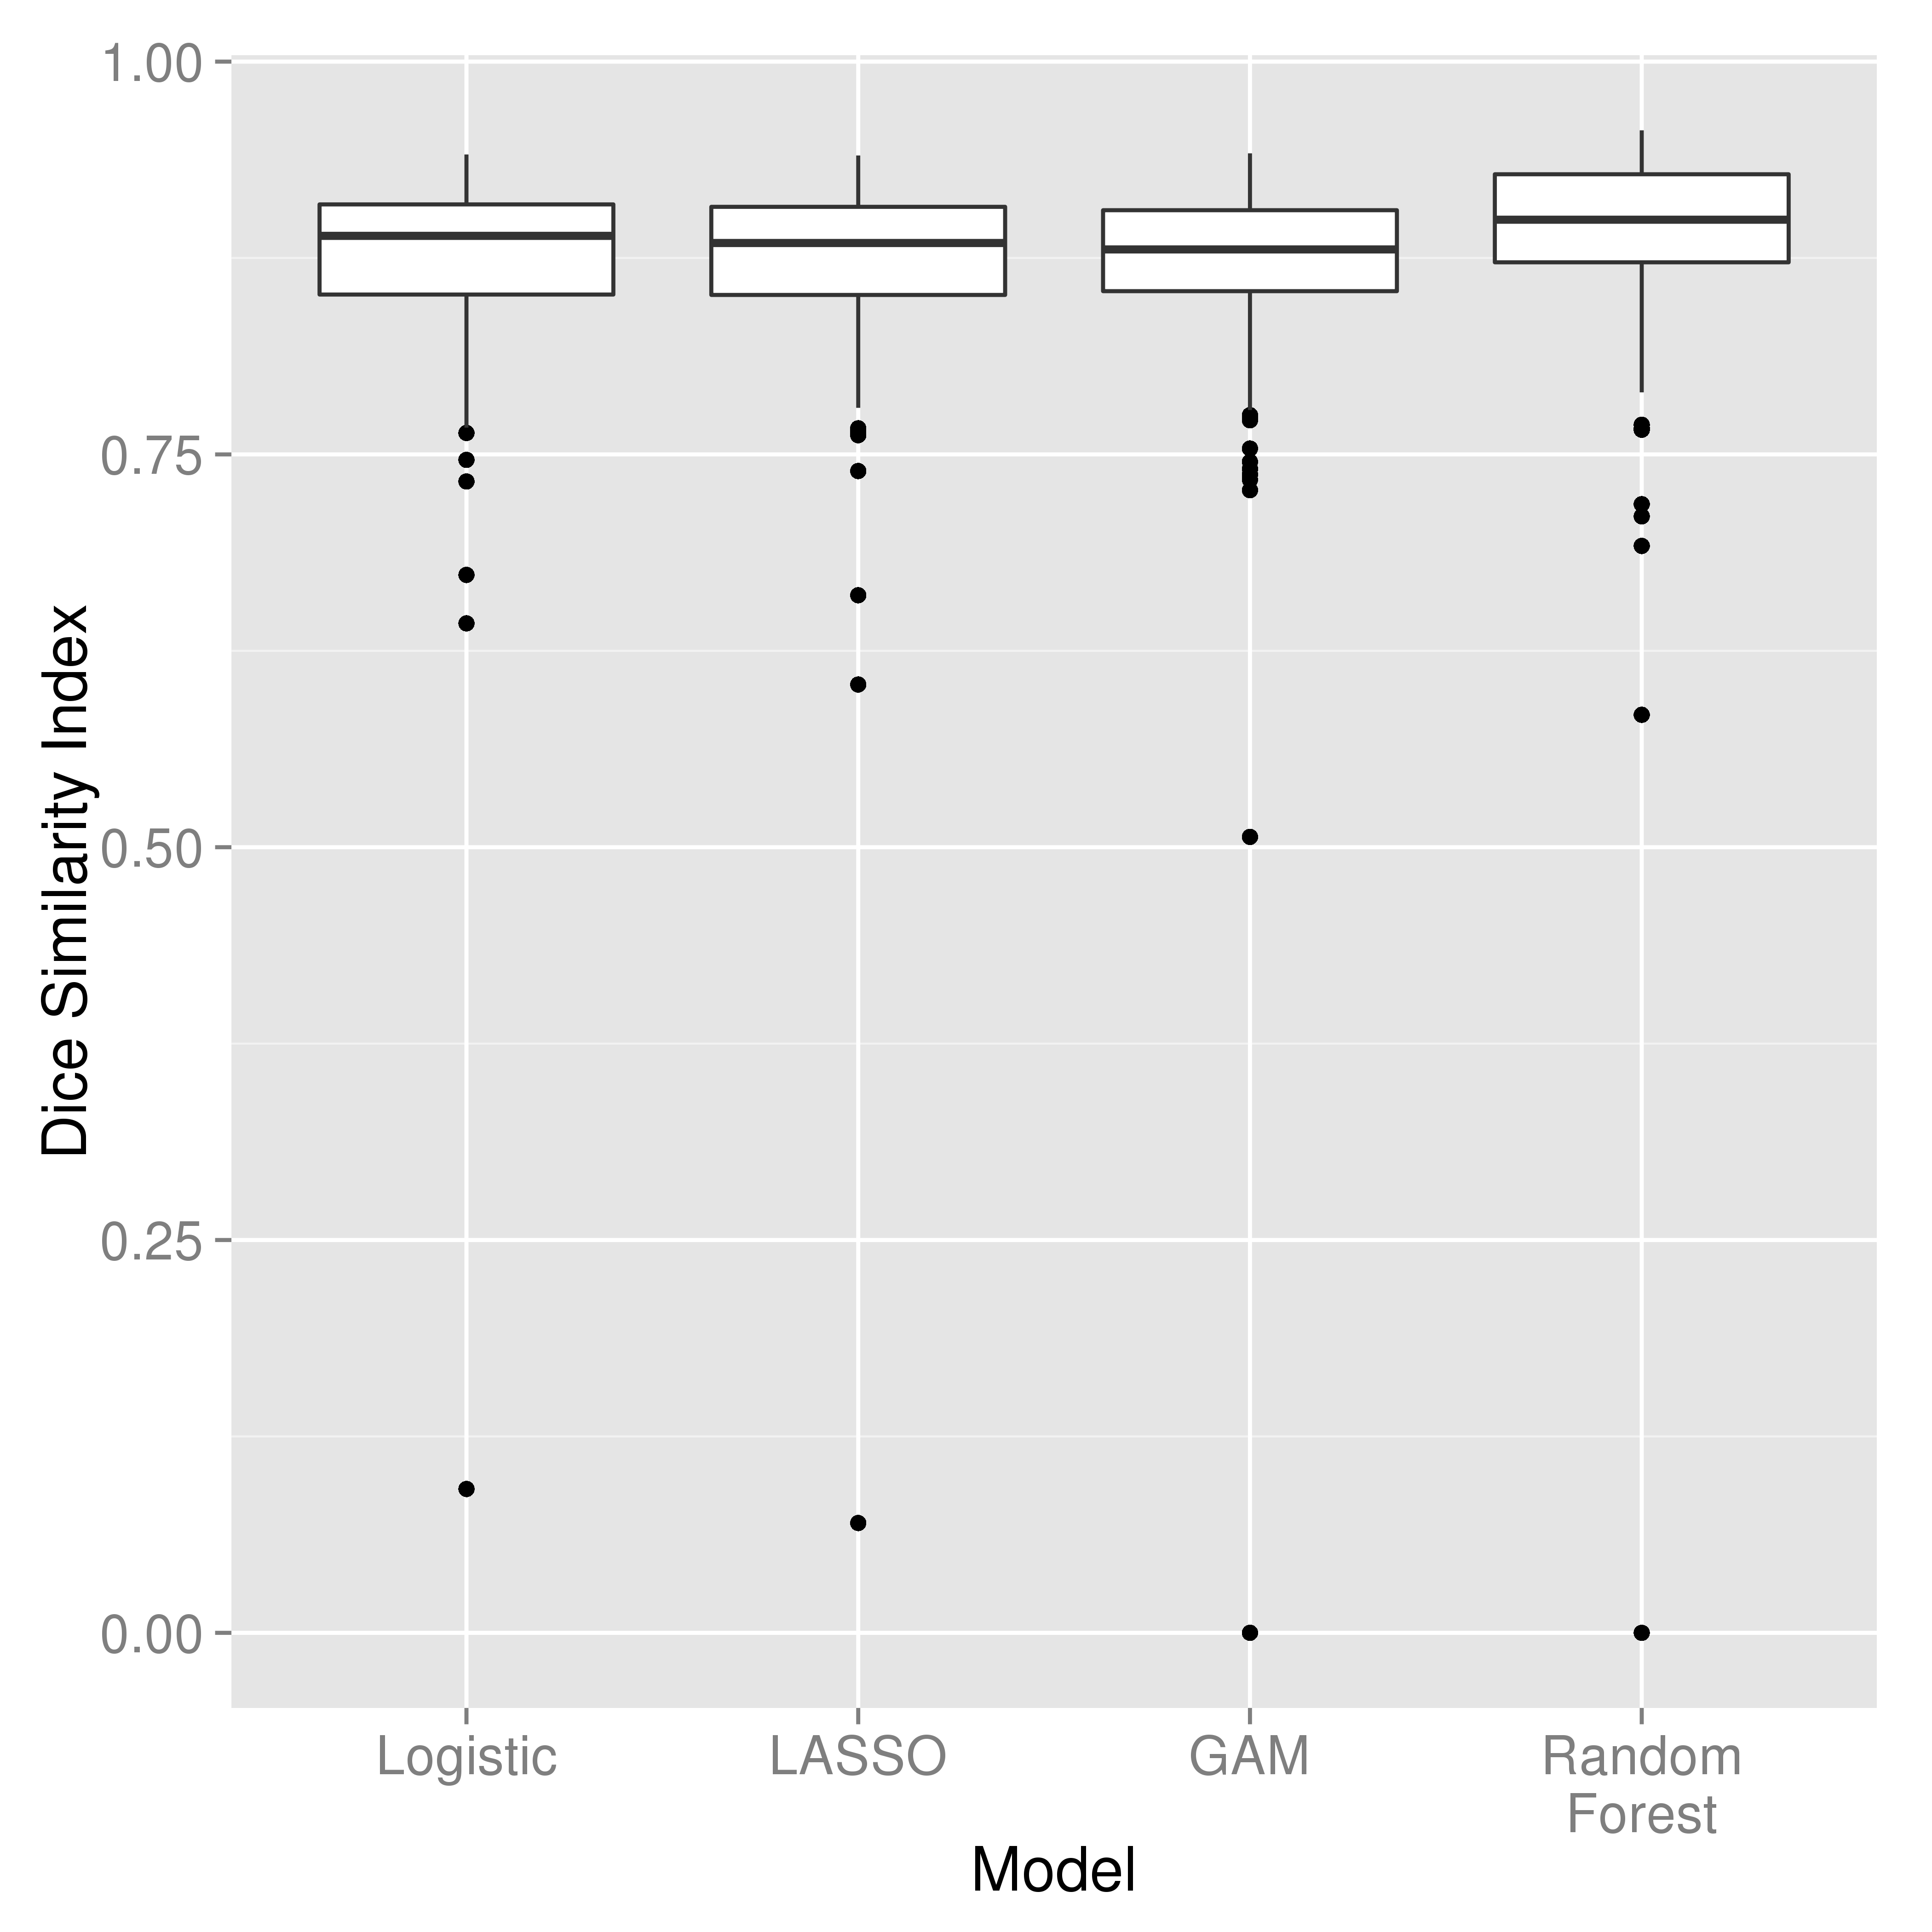
\includegraphics[width=0.75\linewidth,keepaspectratio]{Reseg_Dice_Comparison.png}
\caption{{\bf Distribution of Dice Similarity in Test Scans}.  Here we display the boxplot of the Dice Similarity Index (DSI), a measure of spatial overlap between the estimated hemorrhage mask and the manually delineated hemorrhage mask, in the $102$ test scans.  We present the DSI distribution for each model fit: a logistic regression, a logistic model penalized with the Least Absolute Shrinkage and Selection Operator penalty (LASSO), a generalized additive model (GAM), and a random forest algorithm.  Overall, we see high agreement between the manual and estimated hemorrhage masks with the median of $0.89$ for the logistic model, $0.885$ for the LASSO, $0.88$ for the GAM, and $0.899$ for the random forest. The median DSI for the random forest was significantly higher than those of the other 3 models, after adjusting for multiplicity using a Bonferroni correction (all $p < 0.05$).   }
\label{fig:dice}
\end{figure}



\begin{figure}
\centering
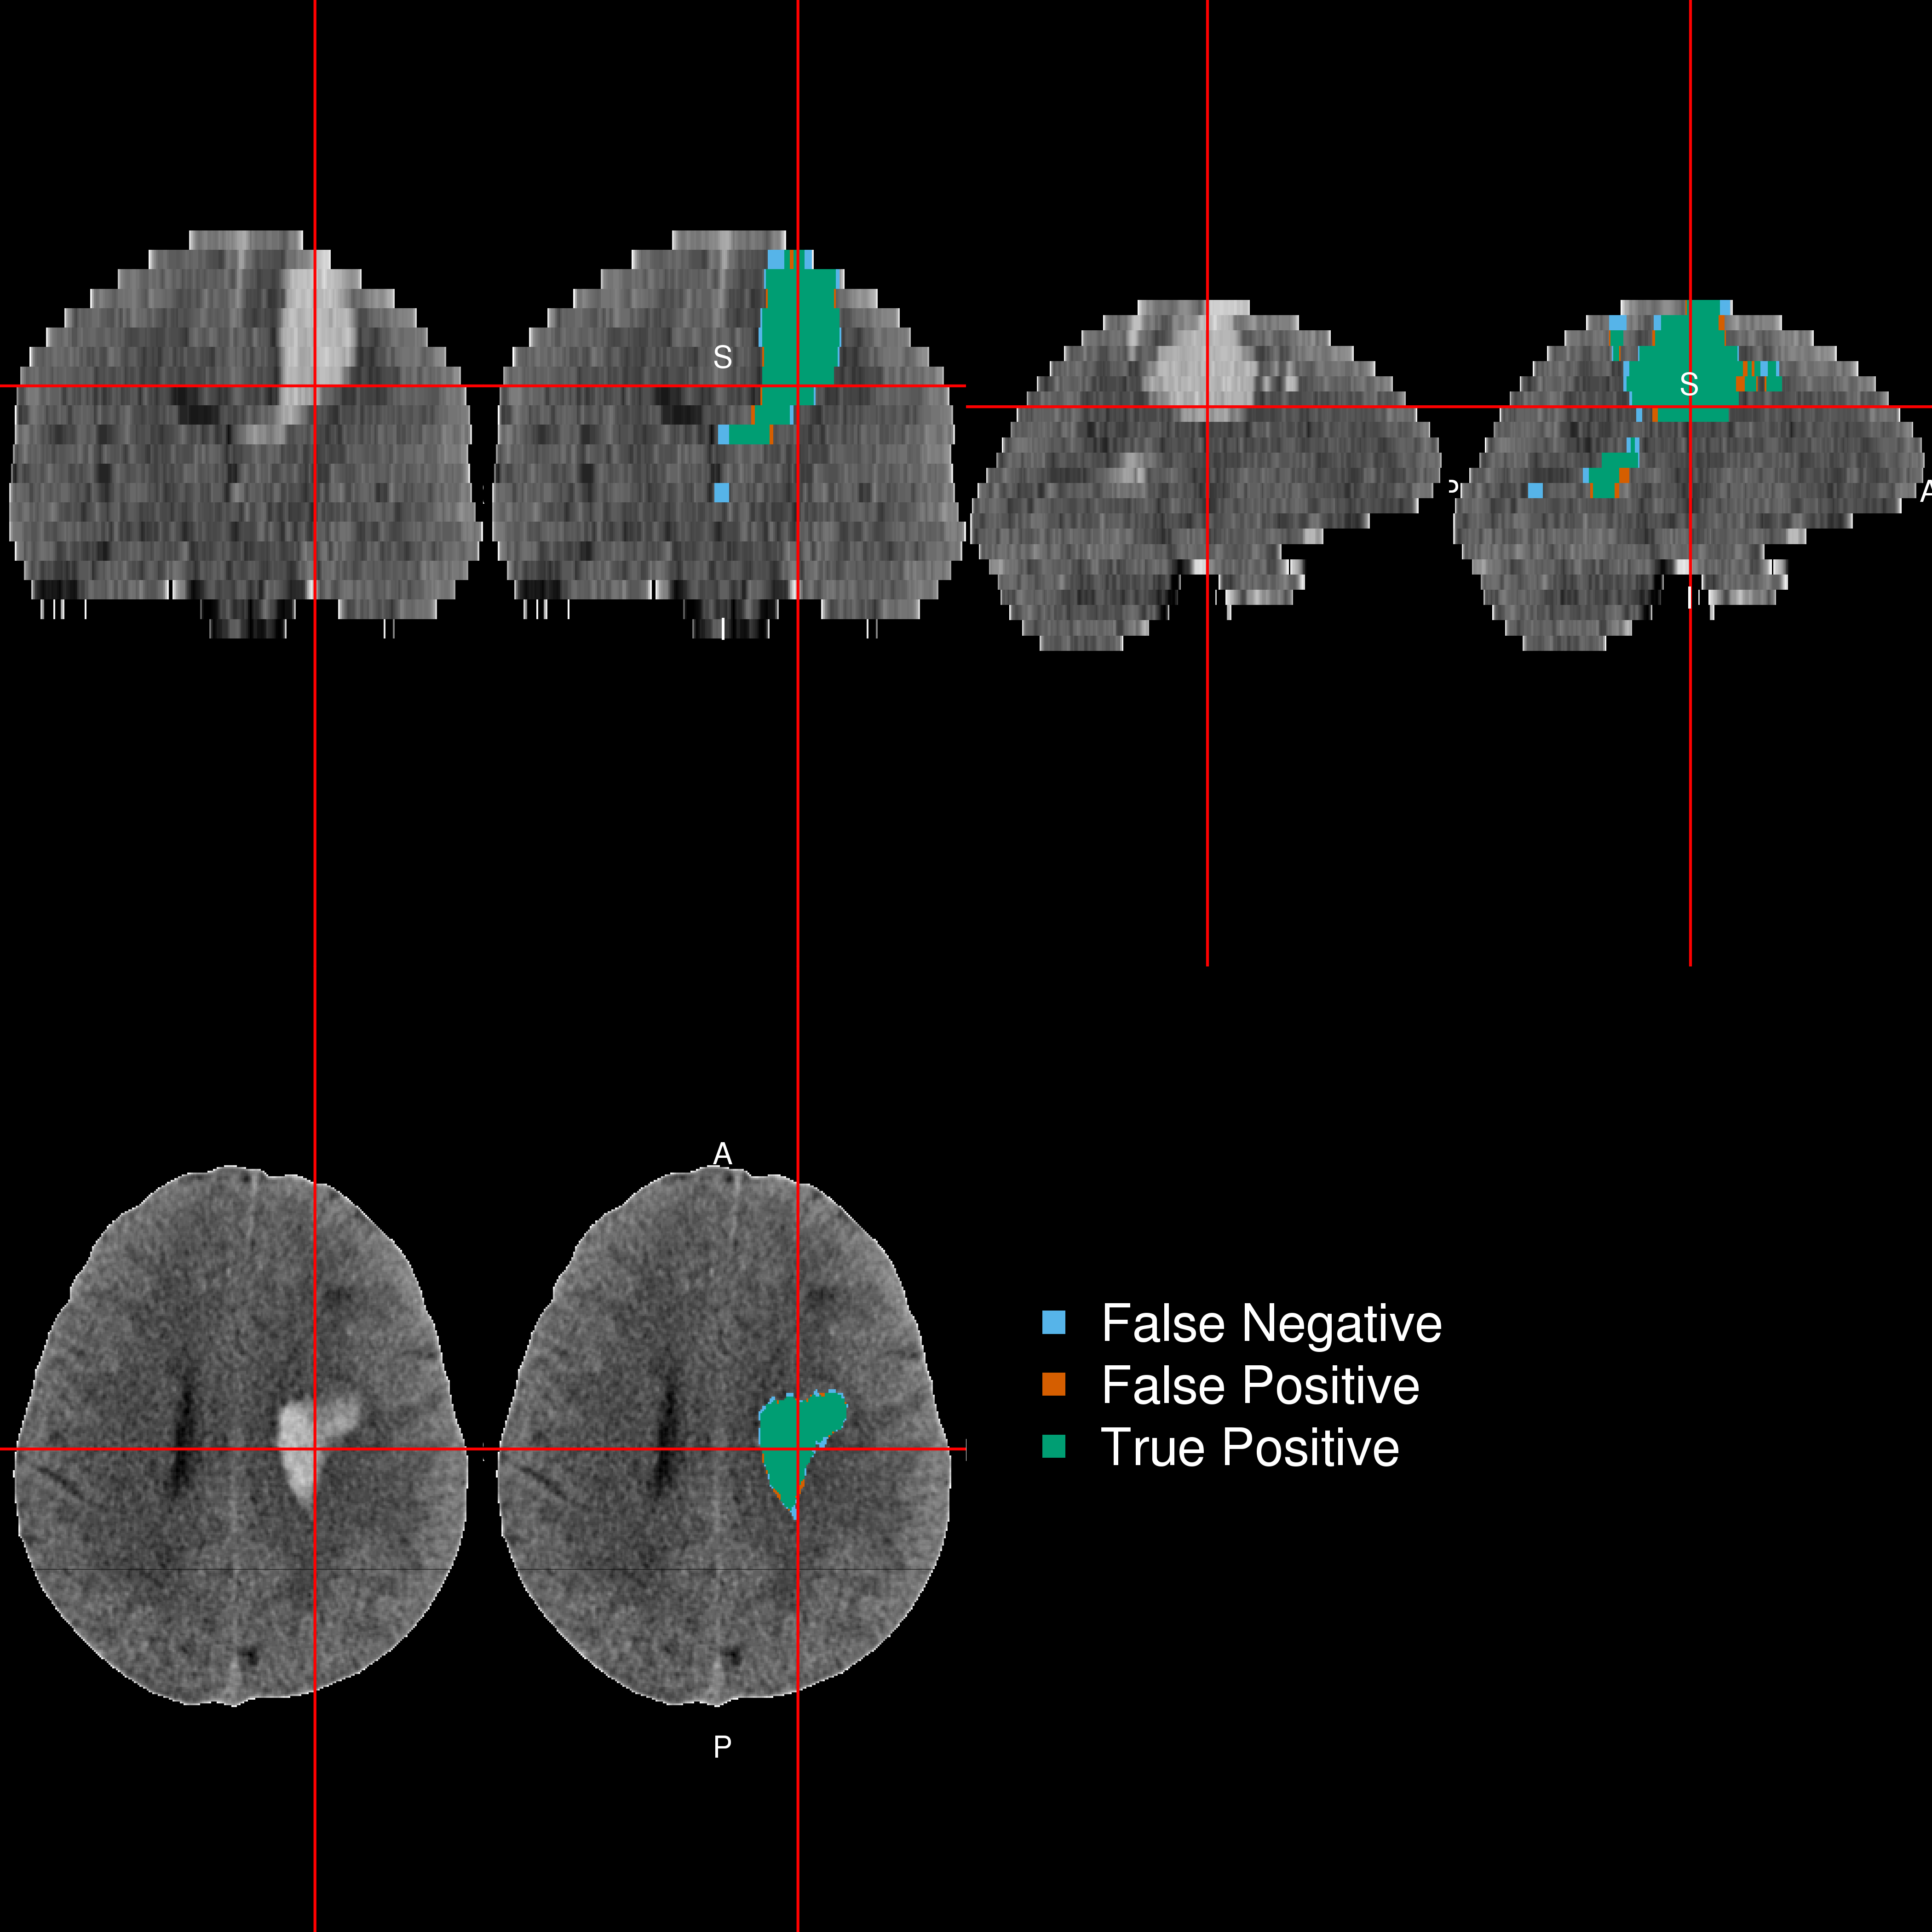
\includegraphics[width=0.75\linewidth,keepaspectratio]{Reseg_Figure_DSI_Quantile_050_native.png}
\caption{{\bf Patient with Median Dice Similarity Index}. We present the patient with the median Dice Similarity Index (DSI), a measure of spatial overlap, from the chosen predictor model fit with a random forest.  The median DSI was $0.899$, which indicates high spatial overlap. The green indicates a correct classification of ICH from the model, blue indicates a false negative, where the manual segmentation denoted the area to be ICH but the predicted one did not, and red indicates a false positive, where the predicted segmentation denoted the area to be ICH but the manual one did not. }
\label{fig:dice_img}
\end{figure}

\subsection{ICH Volume Estimation}
In Figure~\ref{fig:vol}, we show the estimated ICH volume versus that from the manual segmentation.  The pink line represents the $X = Y$ line, where the estimated and true volume are identical.  The blue line represents the linear fit; the estimated linear regression equation and correlation are printed on the plot.  The farther away the slope of the equation is from $1$ the larger the bias with values larger than $1$ representing over-estimated volumes.  
%The farther the intercept is from $0$ represents and additive bias in the estimated volume, where values greater than $0$ again represent larger estimated volumes.  
The correlation (95\% confidence interval (CI)) between the true volume and the predicted volume were $0.92$ (95\% CI: $0.884, 0.945$) for the logistic model, 
$0.916$ ($0.878, 0.942$) for the LASSO, 
$0.908$ (95\% CI: $0.866, 0.937$) for the GAM, and  
$0.932$ (95\% CI: $0.901, 0.954$) for the random forest.  The RMSE for logistic (RMSE: $10.67$ mL), LASSO ($10.83$ mL), and random forest ($10.27$ mL) models were relatively close, but was slightly higher for the GAM model ($11.36$ mL).  The  Kruskal-Wallis test indicated no significant difference in the median absolute value of the difference in estimated versus true volume over models ($\chi^{2}(3)=2.3$, $p = 0.51$).  



\begin{figure}
\centering

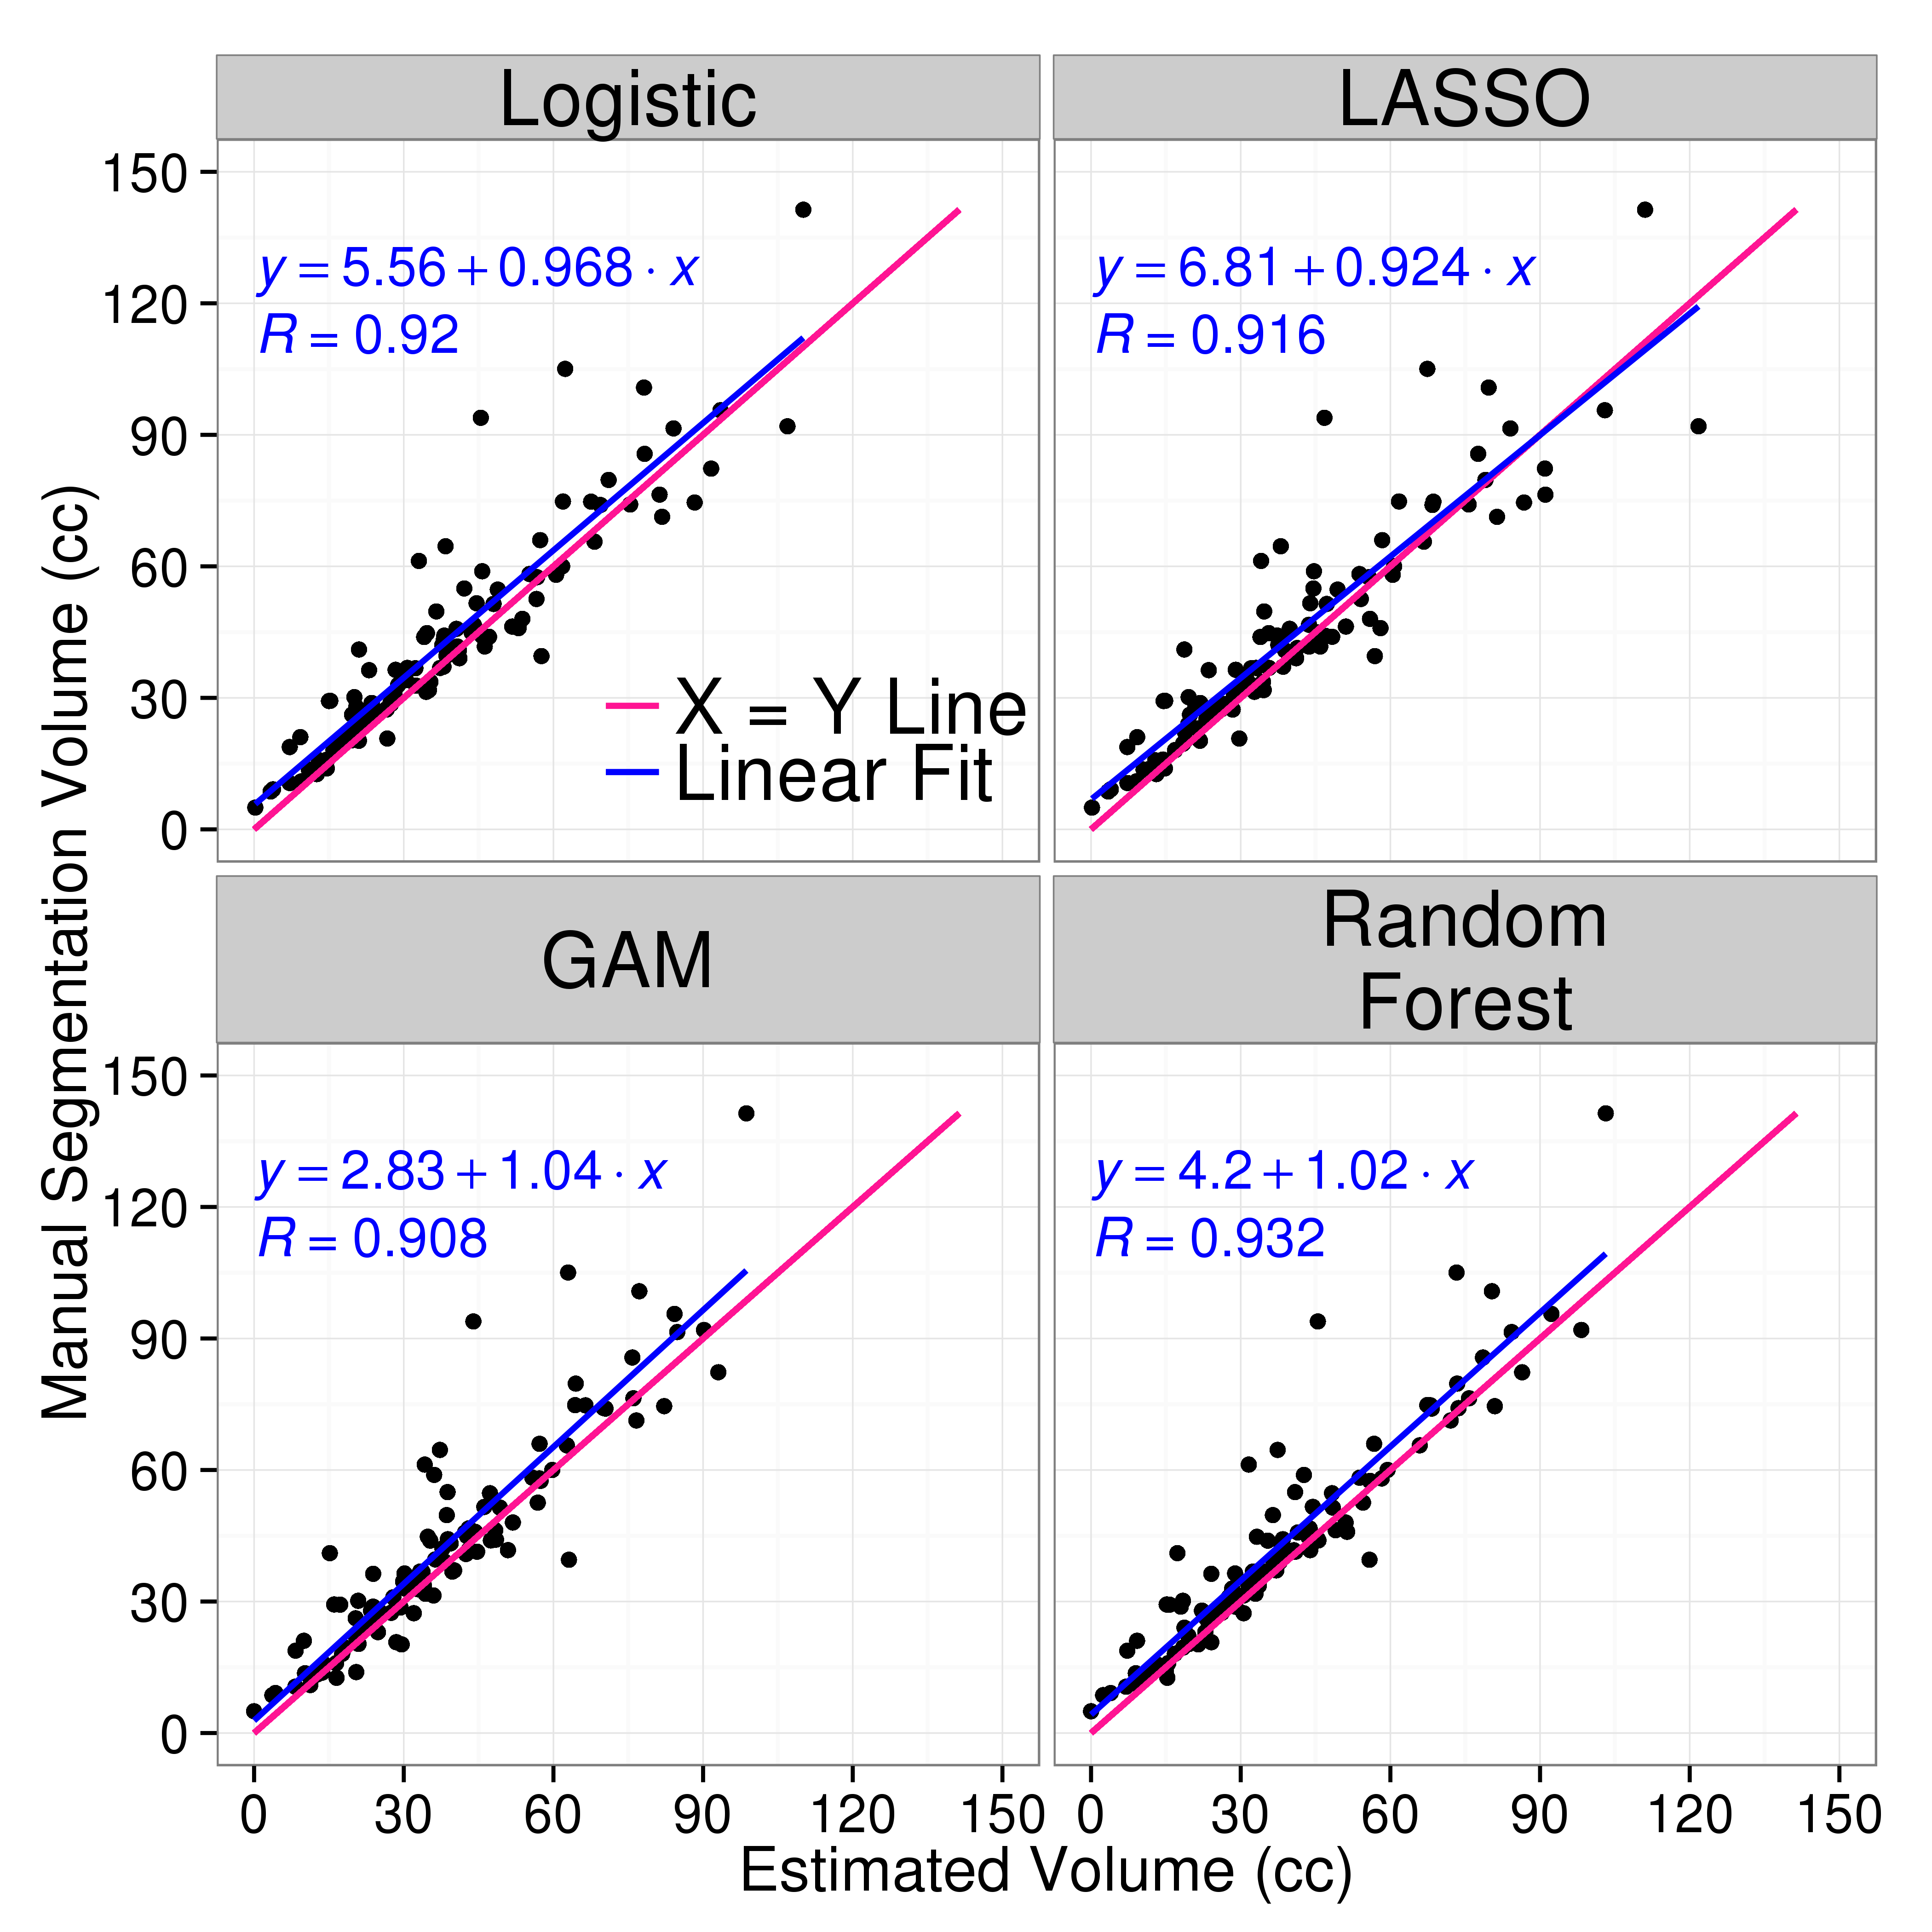
\includegraphics[width=\linewidth,keepaspectratio]{Reseg_Volume_Comparison.png}
\caption{{\bf Comparison of Estimated and Manual Intracerebral Hemorrhage Volume for Each Model}.  In each panel, we show the volume of intracerebral hemorrhage (ICH) estimated from each model (x-axis) versus that from the gold-standard manual segmentation (y-axis) in the $102$ test scans.  The pink line represents the $X=Y$ line, which represents perfect agreement.  The blue line represents a linear fit of the data, and the estimated slope equation is displayed along with the Pearson correlation.  Panel A represents the volume from the logistic regression model, B represents that from logistic model penalized with the LASSO, C represents that from a generalized additive model (GAM), and D represents that from a random forest algorithm.  Overall, we see high agreement between the estimated volumes from automated segmentation from each model as all correlations are above $0.9$.  The farther away the slope of the equation is from $1$ represents a multiplicative bias, where values greater than $1$ represents larger estimated volumes.  The farther the intercept is from $0$ represents and additive bias in the estimated volume, where values greater than $0$ again represent larger estimated volumes.  }
\label{fig:vol}
\end{figure}

\subsection{Model Choice}
Overall, all models perform well for ICH segmentation.  A small percentage ($1.0\%$) of failures were observed with DSI $< 0.5$ ($N = 1$ out of $102$ scans), but the random forest algorithm had a slightly higher median DSI, slightly lower RMSE, and a higher slightly correlation than the other models.  Therefore, when implementing the algorithm, we will use the random forest model.



\section{Discussion}
We have presented a novel, fully automated method for segmentation of ICH from CT scans. Our method uses only CT scans from patients with stroke.  MRI was not 
used because MRI procedures for stroke have not been standardized and are not the standard of care for the disease. We validated this method against the manual segmentation.  We used the Dice Similarity Index and correlation between the volume of ICH from manual and automatic segmentation as measures of algorithm performance.  


To achieve our goal we have started by creating a rich set of predictors that are likely to capture the most discriminating features between ICH and non-ICH voxels and described the rationale for each predictor.  Models of these predictors using logistic regression, logistic regression penalized with the LASSO, generalized additive models, and random forests result in high values for the DSI and high correlations between the total ICH volume obtained from manual and automatic segmentations.  Random forest was chosen as the algorithm, as it slightly outperformed the other approaches on the test data.


The approach failed on a very small ($N = 1$ out of $102$ with DSI below $0.5$). Most discrepancies observed occur at the edges of the hemorrhage.  This may be due to the isotropic, non edge-preserving smoothing.  Anisotropic smoothing, as proposed by \citet{perona1994anisotropic}, may improve segmentation.  



Several other methods have been proposed for segmentation of ICH from CT scans \citep{ gillebert_automated_2014, prakash_segmentation_2012, loncaric_hierarchical_1996, loncaric_quantitative_1999, perez_set_2007}.  \citet{loncaric_hierarchical_1996} performed the analysis on only one 2-dimensional scan and could not be compared with our approach.  The method proposed by \citet{perez_set_2007} is semiautomated and was only validated by visual inspection.  They reported segmentation failure in $6$ out of $36$ scans ($16.7\%$) compared to $1$ out of $102$ scans ($1.0\%$) for our method.   Our reported median DSI ($0.899$) is much larger than the one reported by \citet{gillebert_automated_2014} (approximately $0.62$ and $0.78$ for hemorrhagic strokes as read from their graphs). Our results were comparable to those reported by \citep{prakash_segmentation_2012} ($0.897$, $0.858$, and $0.9173$ for different groups with hemorrhage). \citet{loncaric_quantitative_1999} did not compare hemorrhage and manual segmentation masks; instead they compared ICH volumes from $5$ subjects measured at $3$ timepoints.  Their reported Pearson correlation was $0.917$ for tje $15$ scans, similar to our results using the random forest (R = $0.932$).  

Only \citet{gillebert_automated_2014} responded to our requests for segmentation software to perform the segmentation and we could not find any software online.  Although the method of \citet{gillebert_automated_2014} is comparable to ours, their approach has not been packaged for general use.  We have released an open source package that can perform ICH segmentation (\url{https://github.com/muschellij2/ichseg}).  Our software includes the models for prediction, the CT template from \citet{rorden_age-specific_2012}, template-level standardized mean and standard deviation images, as well as functions to register the images, create the predictors, predict from the models, and return a binary hemorrhage mask.  Although an R package is ideal for prediction on a large number of images and for researchers who prefer scripting, releasing easy to use graphic user interfaces (GUIs) may increase the appeal of the methods proposed. Therefore, we have also released a Shiny \citep{shiny} R application online (\url{http://bit.ly/ICH_SEG}) that takes an input CT scan and outputs ICH segmentation mask and provides a representation of each processing step.  

A potential concerns for CT images that contain ICH is image registration.  Indeed, methods developed for registration of healthy brains can fail in brains exhibiting pathology.  The only predictor that used non-linear registration was the standardized-to-template intensity. The potential problems associated with this transformation are mitigated by the transformation back to the native space. 
%Although this method uses non-linear registration for one predictor, the standardized-to-template intensity, this predictor is transformed back to the rigid-to-template space after standardization.  The method generally relies only rigid-body registration to a template.  This registration is largely done for head reorientation and resampling to isotropic voxel sizes across patients.  Thus, when morphological operations  are performed, such as smoothing using millimeter specifications, they do not depend on the original voxel sizes.  Although the models were fit in the rigid-to-template space, voxels are not compared across patients in the models.  Also, the method returns hemorrhage masks in the native space of the patient, so they are easily comparable to any segmentation method performed on the original scan, such as clustering.  
Thus, we use non-linear registration, but do not rely on a highly accurate image registration to template to compare voxels across patients; instead we use registration to obtain potentially noisy predictors in the native space.

Another potential concern could be that training data consisted of only $10$ patient scans and using only $100{,}000$ randomly sub-sampled voxels that passed the voxel selection procedure from these scans.  Remarkably, the models have shown to have high out-of-sample accuracy.  The training and test sets were kept unchanged to avoid overfitting the models to the test set.  
%If a cross-validation approach was done across the entire set of scans,  the models must also be combined in some way to give a final prediction.  
Validation of the method on additional data would be useful, while rater studies may provide more insight into the clinical differences between various segmentation approaches.  However, we would like to note that our data was highly heterogeneous and contains test scans from multiple sites and scanners. Moreover, the location and size of hemorrhages is also highly heterogeneous.  Thus, we expect our method to have a good out-of-sample accuracy in a heterogeneous population of ICH CT images.

The proposed approach provides estimated binary hemorrhage masks, which can be used to automatically estimate quantitative measures of hemorrhage location \citep{muschelli2015quantitative}.  Our results would also allow automated shape analysis, which require a binary mask.  The subject-specific hemorrhage masks can be used for other voxel-based analyses that could yield novel insights into the relationship between hemorrhage characteristics and patient outcomes.

%Overall, the DSI results indicate good overlap between the predicted ICH segmentation and manual ICH segmentation on average with few failures.  Some non-contiguous areas may not be accurately segmented, but the estimate if ICH volume, which is used in prognostic models for stroke function outcome is accurate.


\subsection{Conclusions}
We have implemented and validated a fully automated segmentation algorithm of ICH in CT scans and published the associated software both as an R package and as a GUI.  The method relies on a series of processing steps and on creating a set of relevant predictors.  This method has been shown to have very good agreement with the gold standard of manual delineation of hemorrhages.  As an automated process, it is much faster, does not require extensive radiologic image experience, is scalable to thousands of images, and does not have inter-reader variability.  As our methods and software produce binary hemorrhage masks that can be localized both in the native and template space \citep{muschelli2015quantitative}, quantitative voxel- and region-level analyses could be conducted to assess the association between ICH characteristics and health outcomes.  Methods also provide an estimator of the ICH volume, which can be used in standard statistical analyses, as it has been shown to be associated with long-term functional outcomes \citep{broderick_volume_1993, jordan2009intracerebral, tuhrim_volume_1999}.  


\section*{Acknowledgments}
We would like to thank the patients and families who volunteered for this study, Genentech Inc. for the donation of the study drug (Alteplase), and the readers who manually segmented the ICH.  Dr. Chris Rorden was also extremely helpful in adapting his \code{dcm2nii} software to some issues specific to CT scans.

\section*{Sources of Funding}
The project described was supported by the NIH grant RO1EB012547 from the National Institute of Biomedical Imaging And Bioengineering, T32AG000247 from the National Institute on Aging, R01NS046309, RO1NS060910, RO1NS085211, R01NS046309, U01NS080824 and U01NS062851 from the National Institute of Neurological Disorders and Stroke, and RO1MH095836 from the National Institute of Mental Health. Minimally Invasive Surgery and rt-PA in ICH Evacuation Phase II (MISTIE II) was supported by grants R01NS046309 and U01NS062851 awarded to Dr. Daniel Hanley from the National Institutes of Health (NIH)/National Institute of Neurological Disorders and Stroke (NINDS).  Minimally Invasive Surgery and rt-PA in ICH Evacuation Phase III (MISTIE III) is supported by the grant U01 NS080824 awarded to Dr. Daniel Hanley from the National Institutes of Health (NIH)/National Institute of Neurological Disorders and Stroke (NINDS). Clot Lysis: Evaluating Accelerated Resolution of Intraventricular Hemorrhage Phase III (CLEAR III) is supported by the grant U01 NS062851 awarded to Dr. Daniel Hanley from the National Institutes of Health (NIH)/National Institute of Neurological Disorders and Stroke (NINDS). 

\newpage
%\section*{References}
%\bibliographystyle{elsarticle-num-names}
%\bibliography{CT_ICH_Segmentation}
%\bibliography{CT_Skull_Stripping_Bib}
\printbibliography

\clearpage
\section{Supplemental Material}

\subsection{Examples of Dice Similarity Index in Test Scans}

\begin{figure}
\centering
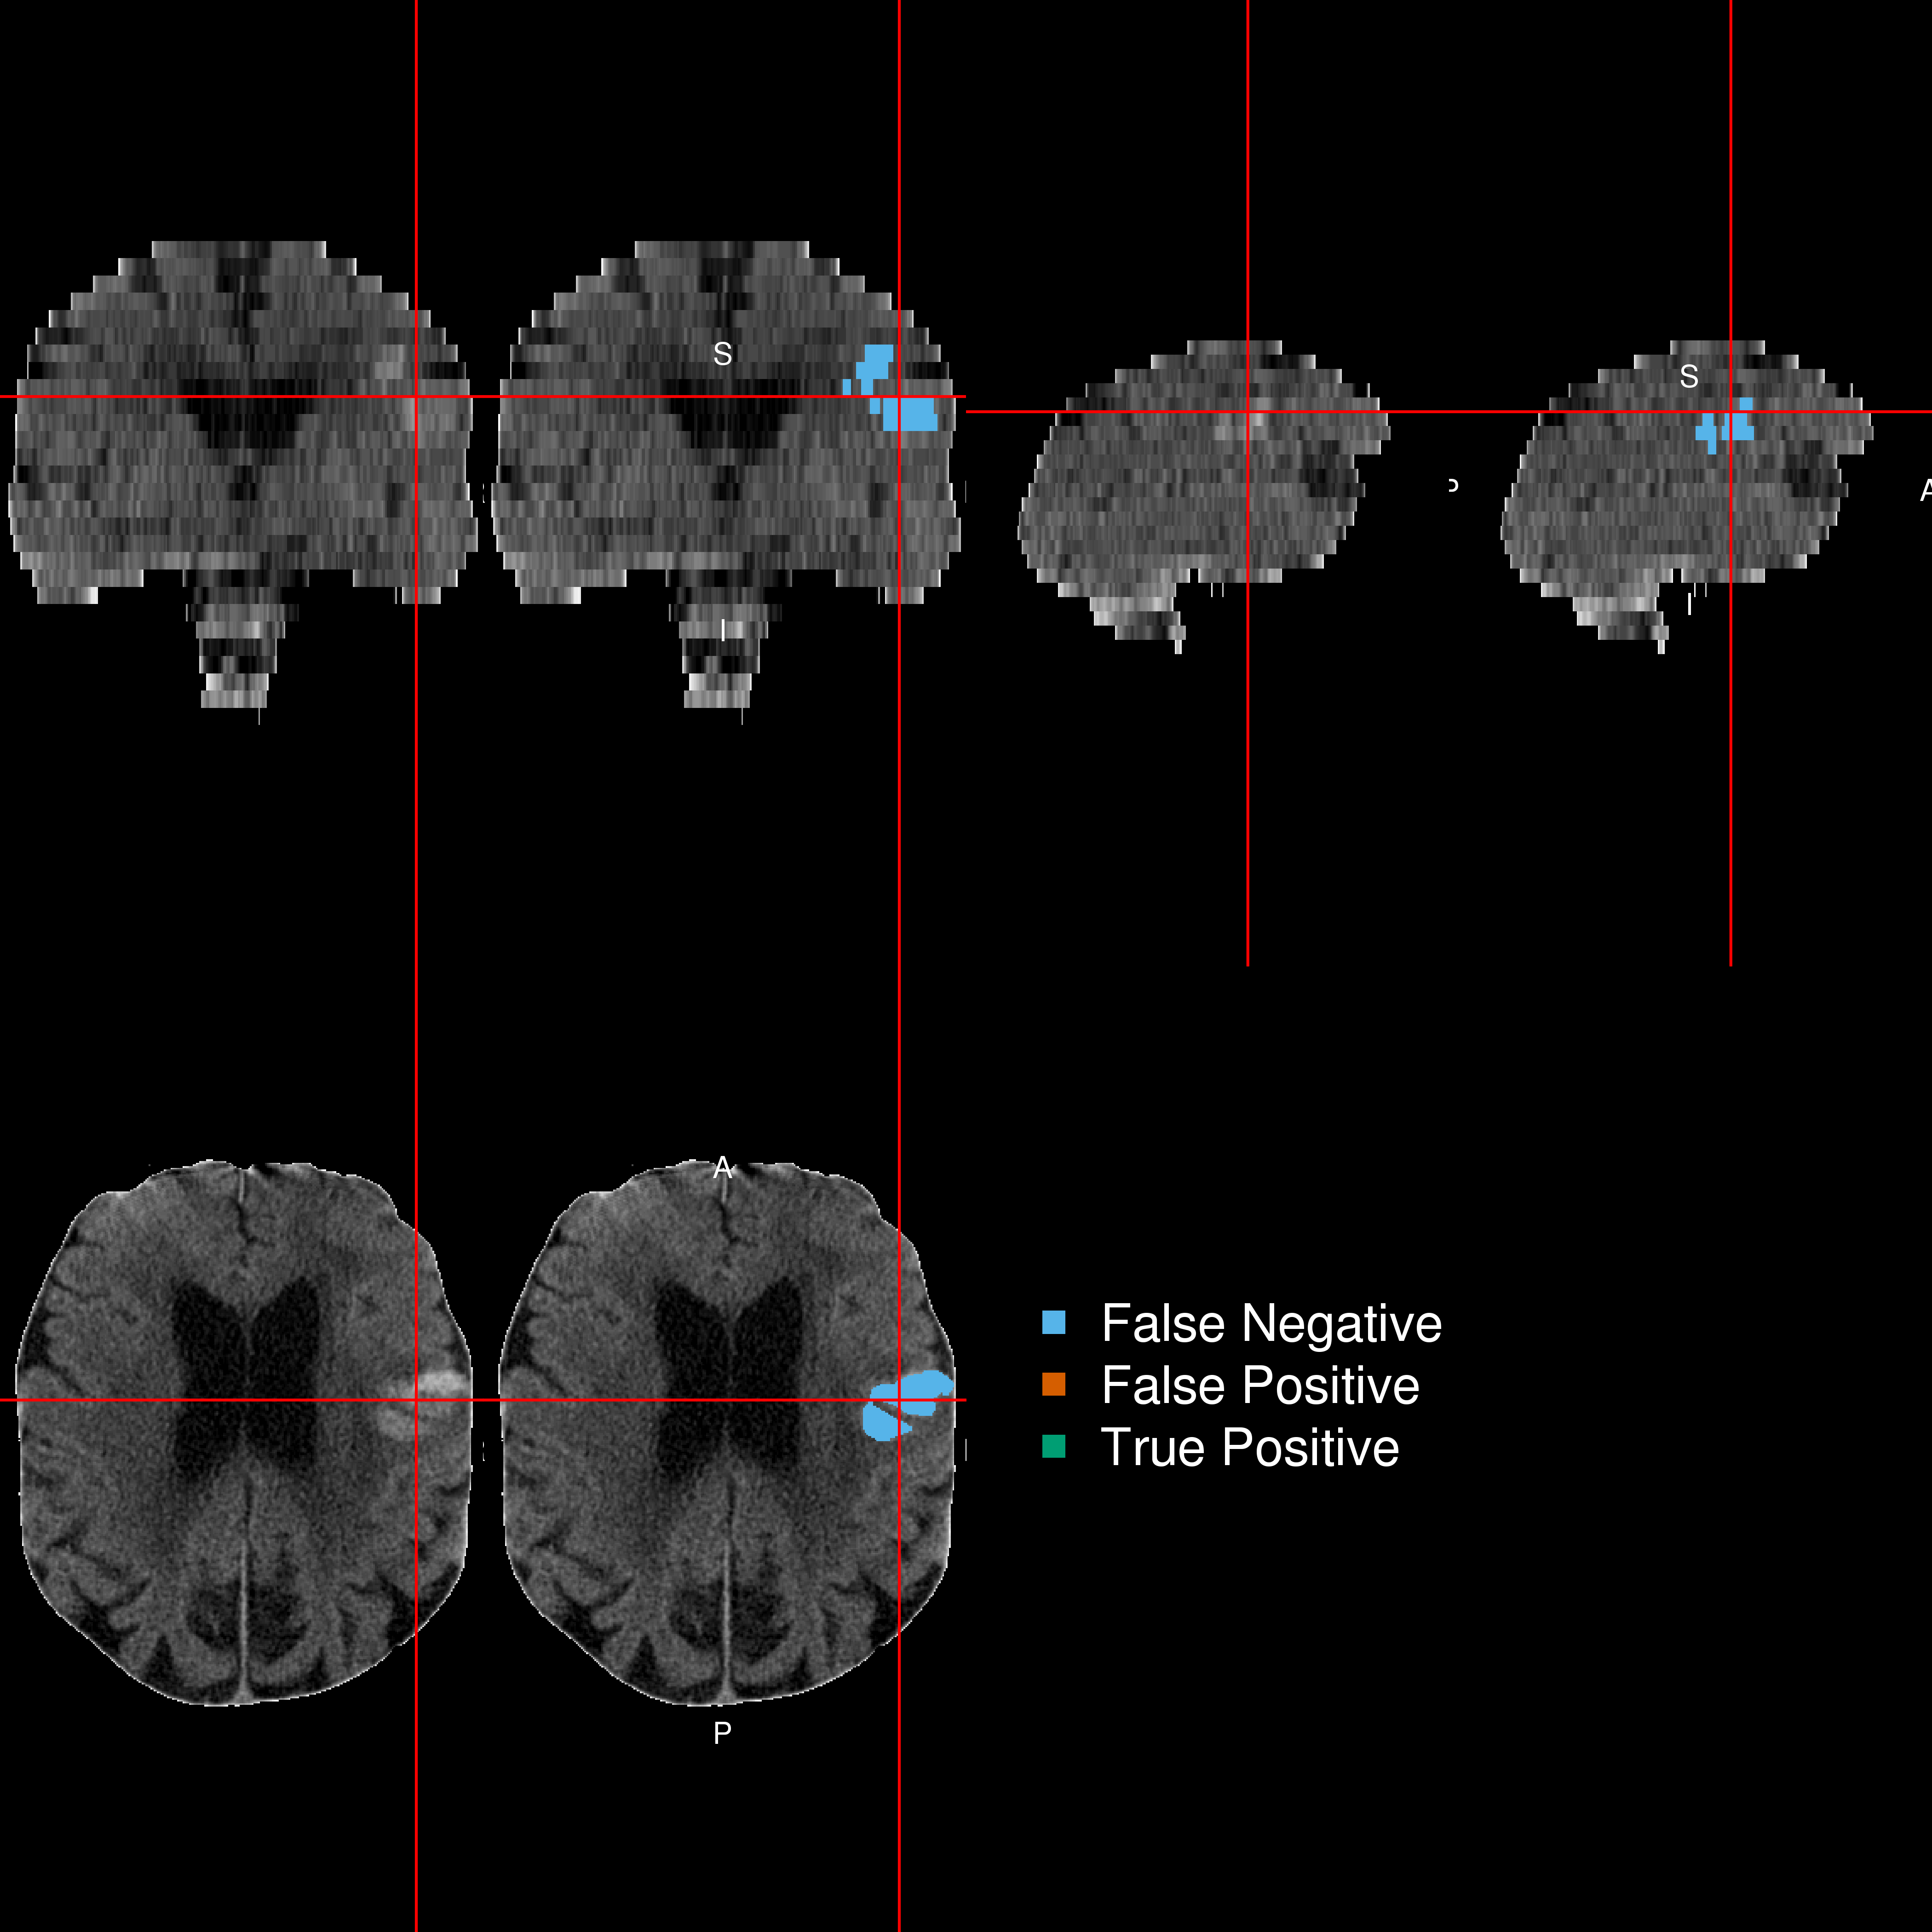
\includegraphics[width=0.75\linewidth,keepaspectratio]{Reseg_Figure_DSI_Quantile_000_native.png}
\caption{{\bf Patient with  Lowest Dice Similarity Index}. We present the patient with the lowest Dice Similarity Index (DSI), a measure of spatial overlap, from the chosen predictor model fit with a random forest.  The lowest DSI was 0. The green indicates a correct classification of ICH from the model, blue indicates a false negative, where the manual segmentation denoted the area to be ICH but the predicted one did not, and red indicates a false positive, where the predicted segmentation denoted the area to be ICH but the manual one did not. }
\label{fig:dice_img0}
\end{figure}

 \begin{figure}
\centering
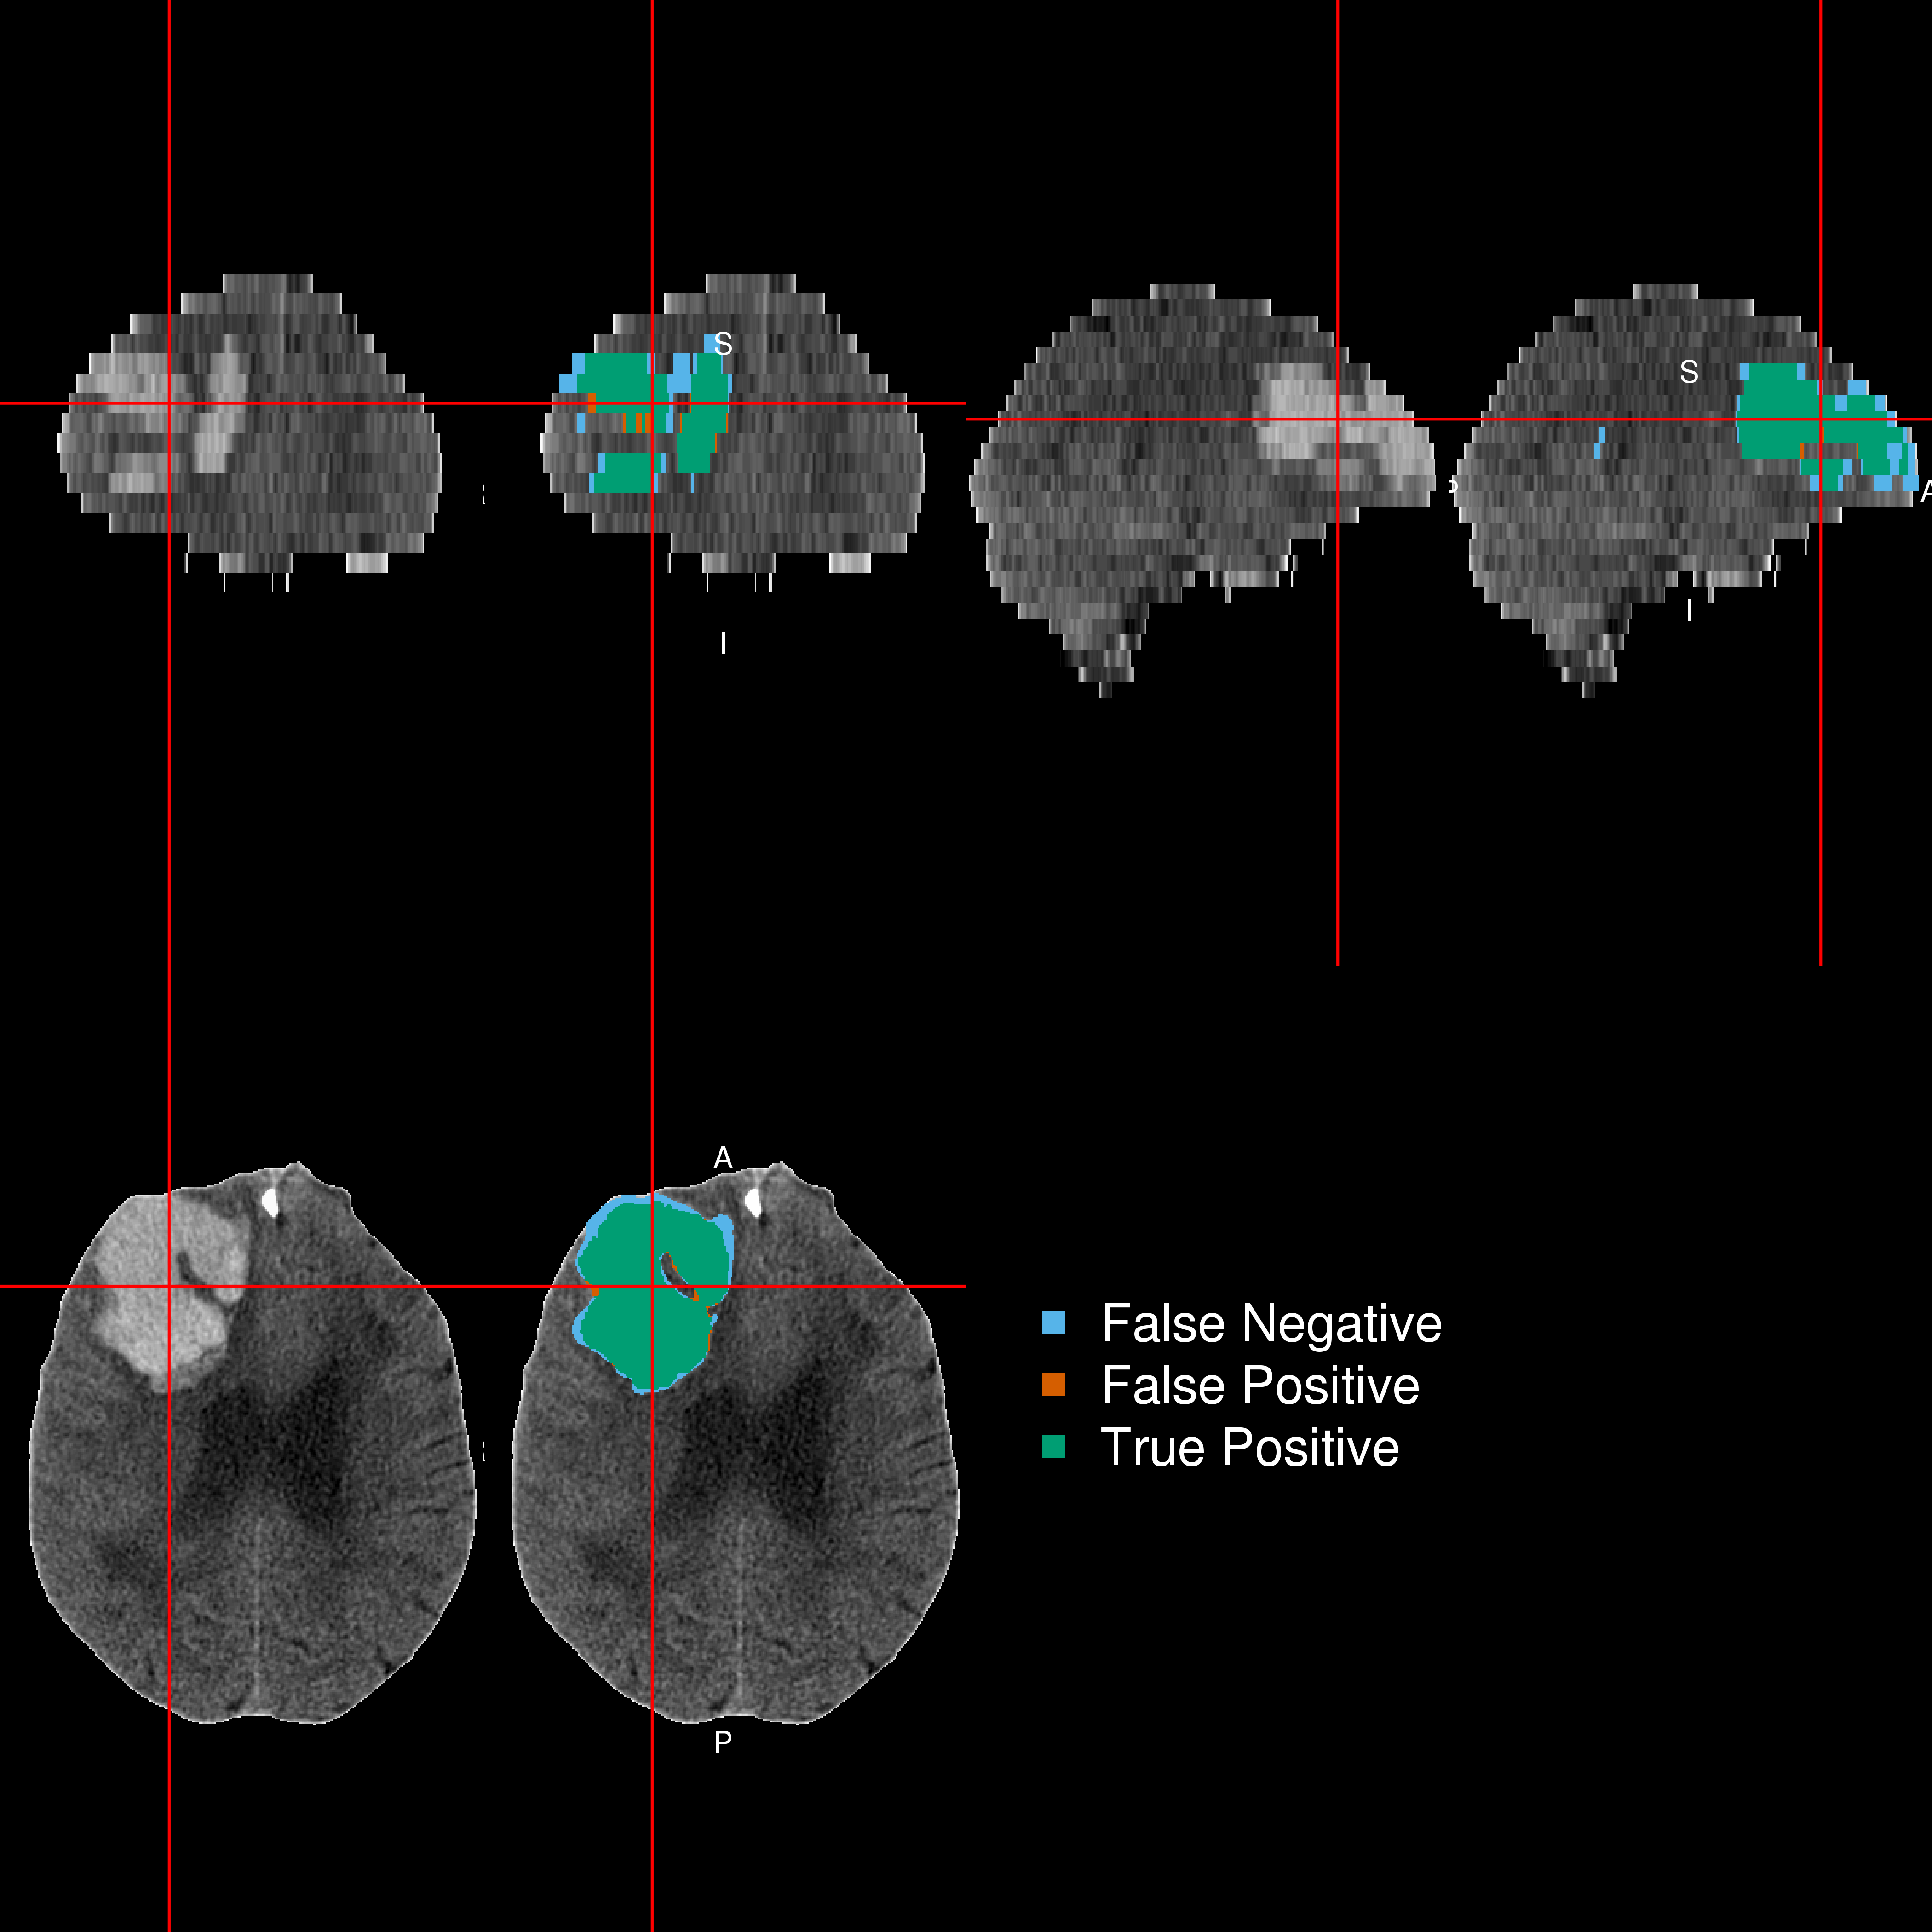
\includegraphics[width=0.75\linewidth,keepaspectratio]{Reseg_Figure_DSI_Quantile_025_native.png}
\caption{{\bf Patient with  25$^{\text{th}}$ Quantile Dice Similarity Index}. We present the patient with the 25$^{\text{th}}$ quantile Dice Similarity Index (DSI), a measure of spatial overlap, from the chosen predictor model fit with a random forest.  The 25$^{\text{th}}$ quantile DSI was 0.872. The green indicates a correct classification of ICH from the model, blue indicates a false negative, where the manual segmentation denoted the area to be ICH but the predicted one did not, and red indicates a false positive, where the predicted segmentation denoted the area to be ICH but the manual one did not. }
\label{fig:dice_img25}
\end{figure}

 \begin{figure}
\centering
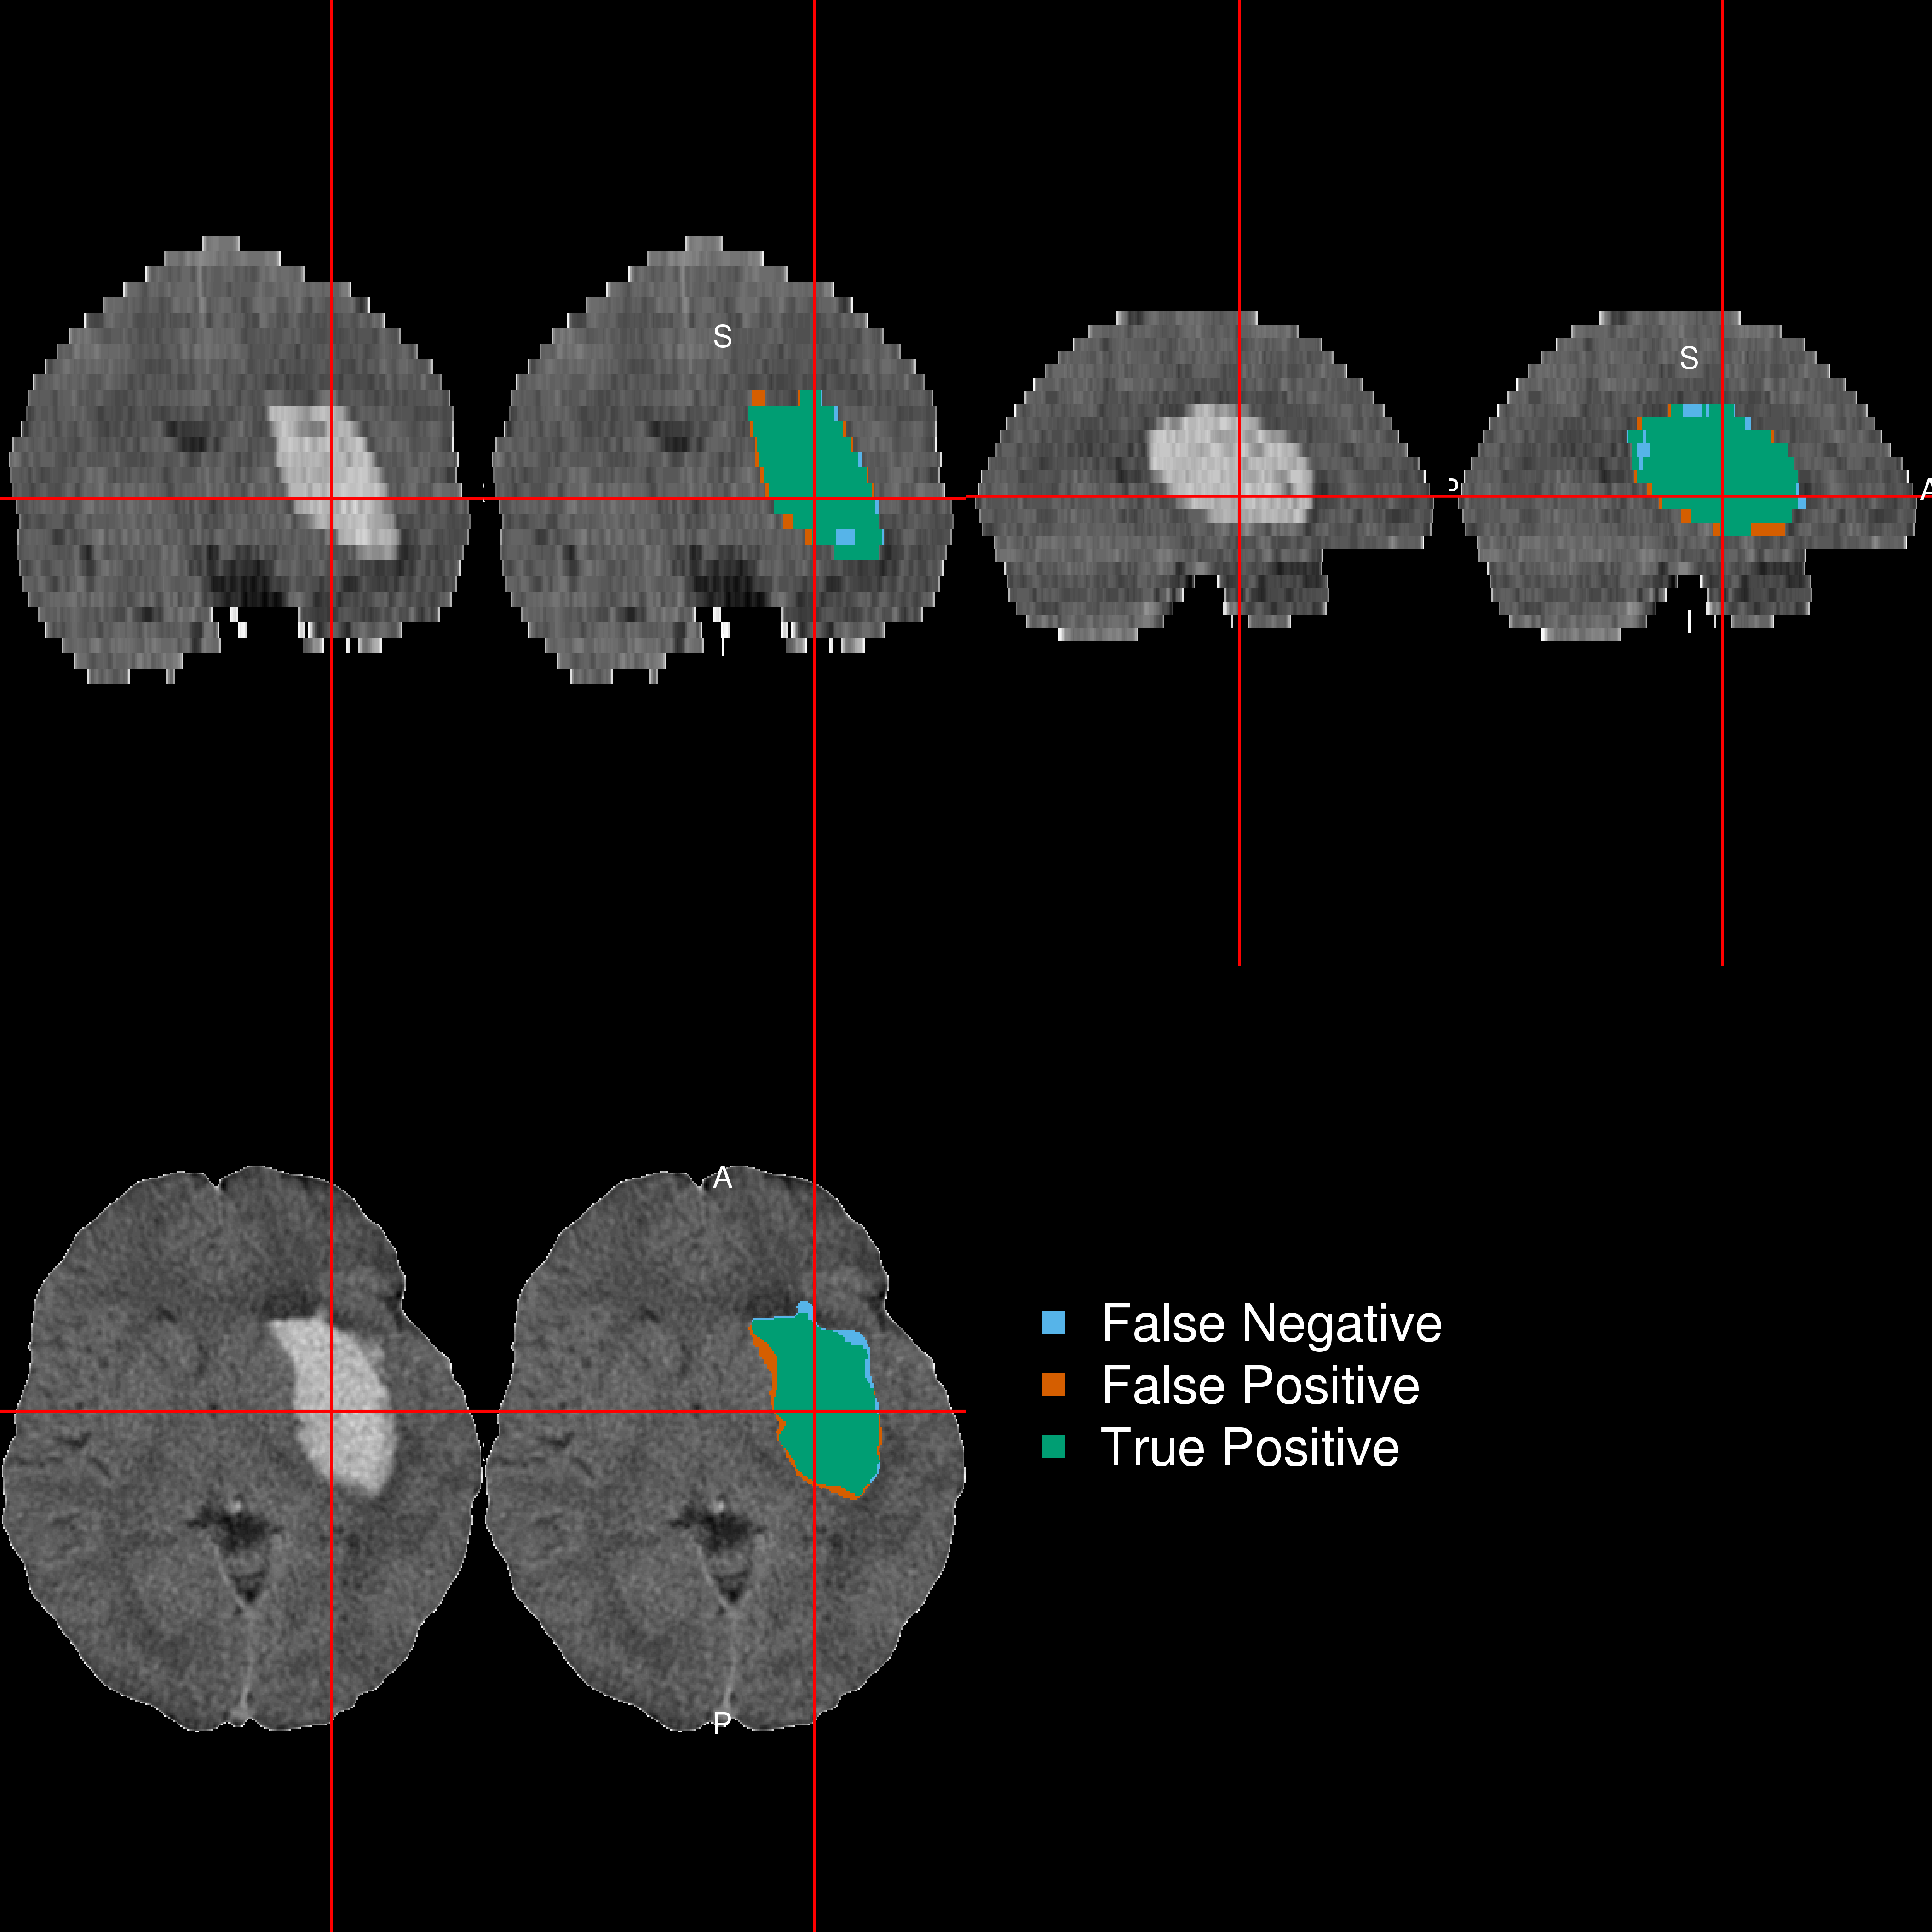
\includegraphics[width=0.75\linewidth,keepaspectratio]{Reseg_Figure_DSI_Quantile_075_native.png}
\caption{{\bf Patient with  75$^{\text{th}}$ Quantile Dice Similarity Index}. We present the patient with the 75$^{\text{th}}$ quantile Dice Similarity Index (DSI), a measure of spatial overlap, from the chosen predictor model fit with a random forest.  The 75$^{\text{th}}$ quantile DSI was 0.928. The green indicates a correct classification of ICH from the model, blue indicates a false negative, where the manual segmentation denoted the area to be ICH but the predicted one did not, and red indicates a false positive, where the predicted segmentation denoted the area to be ICH but the manual one did not. }
\label{fig:dice_img75}
\end{figure}

 \begin{figure}
\centering
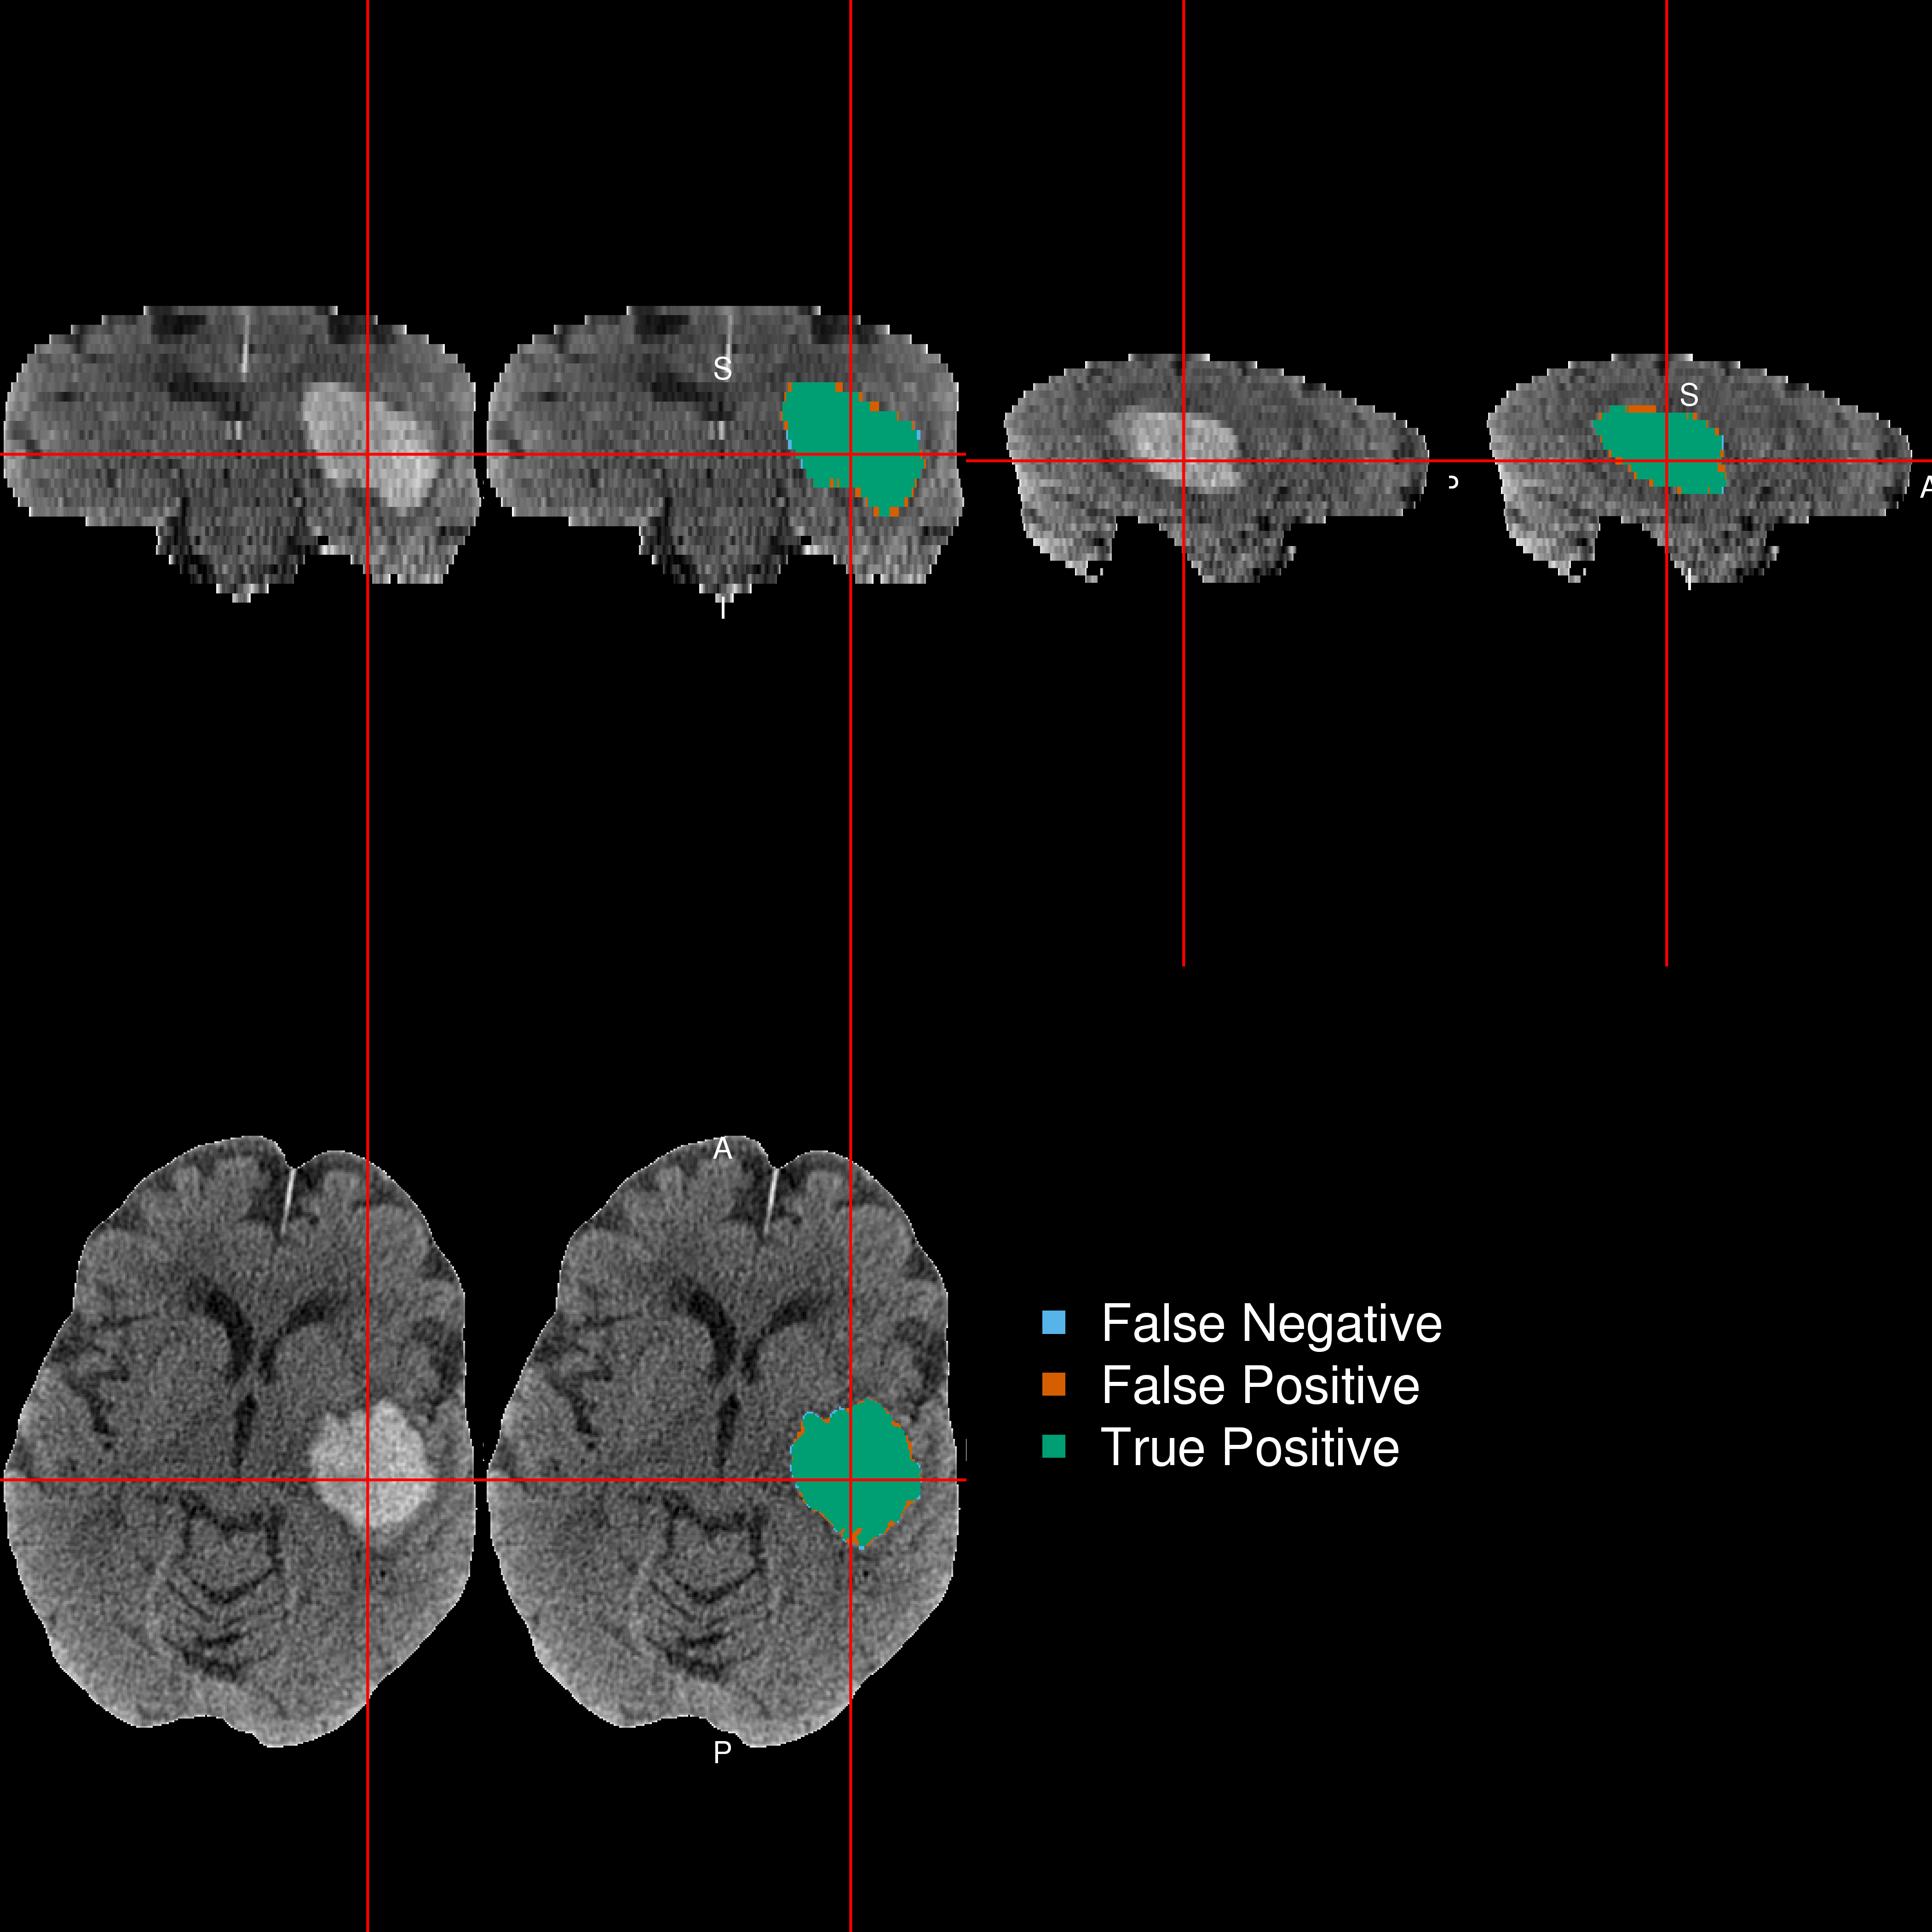
\includegraphics[width=0.75\linewidth,keepaspectratio]{Reseg_Figure_DSI_Quantile_100_native.png}
\caption{{\bf Patient with  Highest Dice Similarity Index}. We present the patient with the highest Dice Similarity Index (DSI), a measure of spatial overlap, from the chosen predictor model fit with a random forest.  The highest DSI was 0.956. The green indicates a correct classification of ICH from the model, blue indicates a false negative, where the manual segmentation denoted the area to be ICH but the predicted one did not, and red indicates a false positive, where the predicted segmentation denoted the area to be ICH but the manual one did not. }
\label{fig:dice_img100}
\end{figure}




\subsection{Model Specification}
\label{sec:modspec}

Let $Y_{i}(v)$ represent the binary hemorrhage mask indicator for voxel $v$, from patient $i$, and $x_{i,v}(k)$ represent the predictor image for image $k$, $k = 1, \dots 21$.
$$
\text{logit}\left(P(Y_{i}(v) = 1)\right) = \beta_0 + \sum_{k = 1}^{21} x_{i, k}(v)\beta_{k}
$$

The coefficients for the logistic model are (in log odds or log odds ratios):

% latex table generated in R 3.3.0 by xtable 1.8-2 package
% Wed Jun  8 16:41:18 2016
\begin{table}[ht]
\centering
\begin{tabular}{lr}
  \hline
Predictor & Beta \\ 
  \hline
Intercept & 1.008 \\ 
  Neighborhood mean & 0.051 \\ 
  Neighborhood sd & 0.000 \\ 
  Neighborhood skew & 0.065 \\ 
  Neighborhood kurtosis & -0.352 \\ 
  Image intensity (HU) & -0.172 \\ 
  Threshold ($\geq$ 40 and $\leq$ 80) & -0.151 \\ 
  Within-plane coronal & -0.632 \\ 
  Within-plane sagittal & -0.249 \\ 
  Within-plane axial & 1.037 \\ 
  Winsorized standardized (20\% trim) & 0.547 \\ 
  Percentage thresholded neighbors & 2.061 \\ 
  Atropos probability image & 0.150 \\ 
  Percent of zero neighbors & -9.180 \\ 
  Indicator of any zero neighbors & 0.071 \\ 
  Distance to image centroid & -0.087 \\ 
  Gaussian smooth ($\sigma = 5$mm$^3$) & -0.051 \\ 
  Gaussian smooth ($\sigma = 10$mm$^3$) & 0.550 \\ 
  Gaussian smooth ($\sigma = 20$mm$^3$) & -0.390 \\ 
  Standardized-to-template intensity & 1.460 \\ 
  Contralateral difference & 0.033 \\ 
   \hline
\end{tabular}
\caption{Beta coefficients (log odds ratio) for the logistic regression model for all coefficients.  Combining these for each voxel value and using the inverse logit transformation yields the probability that voxel is ICH.After smoothing by 1 voxel in all 3 directions, the probability cutoff for thresholding was 0.5481.} 
\label{tab:modspec}
\end{table}


The specification for the functional form of the model fit with the LASSO penalty, is the same, but optimizes the following criteria:
$$
\min_{\beta} - \left( \frac{1}{\sum_{i}V_i} \sum_i Y_{i}(v) \times X_i(v)\beta - \log \left(1 + e^{X_i(v)\beta}\right) \right) +\lambda\sum_{k}\left|\beta_k\right|
$$



\end{document}











